%%=============================================
% !Mode:: "TeX:UTF-8"
% !TEX program  = XeLaTeX
%%=============================================
% 模板名称:hitszthesis
% 模板版本:V3.2.6
% 模板作者:杨敬轩(Jingxuan Yang)
% 联系作者:yangjx20@mails.tsinghua.edu.cn & yanglatex2e@gmail.com
% 模板交流:QQ群:1039392552,加群请备注LaTeX、hitszthesis相关说明
% 模板适用:哈尔滨工业大学(深圳)本、硕、博学位论文
% 模板编译:手动编译方法参看 README.md 或 hitszthesis.pdf
%          GNU make 工具:make thesis
%          Windows 批处理脚本:双击 compile.bat 自动编译论文
%          更多编译细节详见说明文档:hitszthesis.pdf
% 更新时间:2022/12/13
% 模板帮助:请**务必务必务必**阅读 hitszthesis.pdf 说明文档,文档查看方法:
%          cmd 命令行:texdoc hitszthesis
%          推荐前往模板的 GitHub 仓库获取最新文件,地址:
%          https://github.com/YangLaTeX/hitszthesis
%%=============================================

% 设置文档类别为 <hitszthesis>
% \documentclass[type=doctor]{hitszthesis}
%\documentclass[type=master]{hitszthesis}
\documentclass[type=bachelor,infoleft=true]{hitszthesis}

% 模板提供以下选项,各个选项之间不要有空格
% 1. type=bachelor|master|doctor
%   含义:本科、硕士、博士学位论文,不设默认值,**必填**
% 2. covertitletworow=true|false
%   含义:本科封面第一页标题单行或多行显示,默认为单行显示(false)
% 3. infoleft=true|false
%   含义:本科封面第二页下划线内容居中或居左显示,默认为居中显示(false)
% 4. mathfont=newtxmath|mtprotwolite|mtprotwo
%   含义:正文数学字体选项:newtxmath(默认),mtprotwolite(lite版,免费),
%         mtprotwo(完全版,需购买授权),
%         mtpro2字体官网:https://www.pctex.com/mtpro2.html
% 5. boldcaption=true|false
%   含义:图表题注是否加粗,默认为不加粗(false)
% 6. tocfour=true|false
%   含义:是否添加第四级目录,只对本科文科个别要求四级目录有效,默认不添加(false)
% 7. fulltime=true|false
%   含义:是否全日制,非全日制如同等学力等,要在coverinformation中设置类型,
%        默认是全日制(true)
% 8. subtitle=true|false
%   含义:论文题目是否含有副标题,默认没有副标题(false)
% 9. openright=true|false
%   含义:博士论文是否要求章节首页必须在奇数页,默认否(false)
% 10. library=true|false
%   含义:是否为提交到图书馆的电子版,默认否(false)
% 11. alphappendix=true|false
%   含义:本科毕业设计附录章节编号是否为大写字母,默认是(true)
% 12. bsfrontpagenumberline=true|false
%   含义:本科毕业设计前言部分页码是否添加短横线,默认是(true)
% 13. bsmainpagenumberline=true|false
%   含义:本科毕业设计正文部分页码是否添加短横线,默认是(true)

% 自定义设置与额外加载的宏包请写在 \file{hitszthesis.sty} 里
\usepackage{hitszthesis}

% 图片存放路径,在这些文件夹里的图片可以直接使用图片文件名调用
\graphicspath{{figures/}{pictures/}}

%%=============================================
% 开始写论文
% !!注意本文仅作为排版格式示例,并不作为毕业论文规范
\begin{document}

% 开始写前言部分
\frontmatter

% 封面信息填写
% !TEX root = ../main.tex

% 专硕请取消下面注释
% \makeatletter
%   \def\hitsz@csubjecttitle{类别}
% \makeatother

\hitszsetup{
  %******************************
  % 注意:
  %   1. 配置里面不要出现空行
  %   2. 不需要的配置信息可以删除
  %******************************
  %
  %=====
  % 秘级
  %=====
  statesecrets={公开},
  natclassifiedindex={TM301.2},
  intclassifiedindex={62-5},
  %
  %=========
  % 中文信息
  %=========
  ctitleone={高性能RISC-V开源处理器虚拟化},%本科生封面使用
  ctitletwo={虚拟化扩展与系统评测},%本科生封面使用
  ctitlecover={高性能RISC-V开源处理器\\虚拟化扩展与系统评测},%放在封面中使用,自由断行
  ctitle={高性能RISC-V开源处理器虚拟化扩展与系统评测},%放在原创性声明中使用
  % csubtitle={一条副标题}, %一般情况没有,可以注释掉
  cxueke={工学},
  cpostgraduatetype={学术},
  csubject={计算机科学与技术},
  % csubject={机械工程},
  caffil={计算学部},
  % caffil={哈尔滨工业大学(深圳)},
  cauthor={胡光辉},
  csupervisor={黄庆成 副教授},
  % cassosupervisor={某某某 教授}, % 副导师
  % ccosupervisor={某某某 教授}, % 合作导师
  % 日期自动使用当前时间,若需指定按如下方式修改:
  cdate={2022年6月},
  % 指定第二页封面的日期,即答辩日期
  cdatesecond={2022年06月09日},
  cstudentid={SZ160310217},
  cstudenttype={同等学力人员}, %非全日制教育申请学位者
  %(同等学力人员)、(工程硕士)、(工商管理硕士)、
  %(高级管理人员工商管理硕士)、(公共管理硕士)、(中职教师)、(高校教师)等
  %
  %
  %=========
  % 英文信息
  %=========
  etitle={Research on key technologies of partial porous externally pressurized gas bearing},
  esubtitle={This is the sub title},
  exueke={Engineering},
  esubject={Mechanical Engineering},
  eaffil={Harbin Institute of Technology, Shenzhen},
  eauthor={Jingxuan Yang},
  esupervisor={Prof. XXX},
  % eassosupervisor={XXX},
  % ecosupervisor={Prof. XXX}, % Co-Supervisor off Campus
  % 日期自动生成,若需指定按如下方式修改:
  edate={June, 2022},
  estudenttype={Master of Engineering},
  %
  % 关键词用“英文逗号”分割
  ckeywords={\TeX, \LaTeX, CJK, 论文模板, 毕业论文},
  ekeywords={\TeX, \LaTeX, CJK, hitszthesis, thesis},
}

% 中文摘要
\begin{cabstract}

  摘要是论文内容的高度概括,应具有独立性和自含性,即不阅读论文的全文,就能获得必要的信息。摘要应包括本论文的目的、主要研究内容、研究方法、创造性成果及其理论与实际意义。摘要中不宜使用公式、化学结构式、图表和非公知公用的符号与术语,不标注引用文献编号,同时避免将摘要写成目录式的内容介绍。

  关键词是为了文献标引工作、用以表示全文主要内容信息的单词或术语。关键词不超过5个,每个关键词中间用分号分隔。(模板作者注:关键词分隔符不用考虑,模板会自动处理。英文关键词同理。)

\end{cabstract}

% 英文摘要
\begin{eabstract}

  Externally pressurized gas bearing has been widely used in the field of aviation, semiconductor, weave, and measurement apparatus because of its advantage of high accuracy, little friction, low heat distortion, long life-span, and no pollution. In this thesis, based on the domestic and overseas researching\dots\dots

  Key words are terms used in a dissertation for indexing, reflecting core information of the dissertation. An abstract may contain a maximum of 5 key words, with semi-colons used in between to separate one another.

\end{eabstract}


% 生成封面、中英文摘要
\makecover

% 物理量名称表,若采用标准符号则不需要此表
% % !TEX root = ../main.tex

% 物理量符号表,如果采用标准符号则不需要此表
\begin{denotation}
  % 此处最好是h
  \begin{table}[h]
  \caption{国际单位制中具有专门名称的导出单位}
  \vspace{0.5em}\centering\wuhao
  \begin{tabular}{ccccc}
    \toprule[1.5pt]
    量的名称&单位名称&单位符号&其它表示实例\\
    \midrule[1pt]
    频率&赫[兹]&Hz&s-1\\
    \bottomrule[1.5pt]
    \end{tabular}
  \end{table}
\end{denotation}


% 中文目录
\tableofcontents

% 英文目录,本硕不要求
% \tableofengcontents

% 开始写正文
\mainmatter

% 第1章
% !TEX root = ../main.tex

% 中英标题:\chapter{中文标题}[英文标题]
\chapter{绪论}[Introduction]

\section{课题背景及研究的目的和意义}[Background, objective and significance of the subject]

虚拟化是一项重要的计算机技术,为云数据中心各类服务提供关键技术支撑。
近年来,云数据中心和云服务提供商发展迅速。
从传统的虚拟机和容器,到新兴的函数服务(Function as a service)和无服务计算(serveless),
都有着巨大的需求和广阔的发展前景。
这不断推动着虚拟化技术的发展,特别是处理器虚拟化技术。
处理器虚拟化技术作为虚拟化中硬件兼容性最完整的一项技术,
能够使虚拟机可以运行与底层硬件完全不同的操作系统,在云服务中发挥着重要作用。

多年来,在需求的刺激下,关于虚拟化技术和评测手段的研究,特别是x86和ARM架构,已经相当成熟。
但是RISC-V,作为一个新兴的、开源的精简指令集,其处理器虚拟化技术的研究尚未完全展开,还有巨大的研究空间。
由于具有简洁、高效、模块化的特点,RISC-V在计算机体系结构领域中受到了学术界和工业界广泛关注。
为了实现处理器虚拟化,RISC-V基金会于2021.12月提出一个指令集扩展:虚拟化扩展(Hypervisor Extension)。
虚拟化扩展作为指令集架构的子集,规定了实现处理器虚拟化必须添加的硬件功能,包括特权指令和页表翻译等。

关于RISC-V虚拟化扩展的研究,加州大学的伯克利分校迈出了第一步。
他们研发了Rocket Chip,一个开源的RISC-V顺序流水线处理器,
并在其上实现了完整的虚拟化扩展,进行了一系列虚拟化相关的评测。
但是在真实应用场景下,硬件情况会更为复杂,
多核乱序的处理器核心才是虚拟化服务器的主流。
关于这方面的研究尚未完全展开,亟待进行。



\section{本文的主要研究内容}
该项目主要研究对象是RISC-V开源处理器,研究内容是硬件虚拟化实现和评测。
本课题瞄准XiangShan项目的“南湖”架构处理器。
XiangShan是由中国科学院计算技术研究所牵头发起高性能开源RISC-V处理器项目,
是目前国际上性能最高的开源高性能 RISC-V 处理器核。
而“南湖”则是一个较为稳定的用于学术研究的版本。

% 第2章
% !TEX root = ../main.tex

% 中英标题:\chapter{中文标题}[英文标题]
\chapter{“南湖”处理器虚拟化扩展的设计与实现}[Typesetting pictures]

\section{引言}[Introduction]
图应有自明性。插图应与文字紧密配合,文图相符,内容正确。选图要力求精练,插图、照
片应完整清晰。机械工程图:采用第一角投影法,严格按照GB4457~GB131-83《机械制图》
标准规定。数据流程图、程序流程图、系统流程图等按GB1526-89标准规定。电气图:图形
符号、文字符号等应符合附录3所列有关标准的规定。流程图:必须采用结构化程序并正确
运用流程框图。对无规定符号的图形应采用该行业的常用画法。坐标图的坐标线均用细实线
,粗细不得超过图中曲线;有数字标注的坐标图,必须注明坐标单位。照片图要求主题和主
要显示部分的轮廓鲜明,便于制版。如用放大或缩小的复制品,必须清晰,反差适中。照片
上应有表示目的物尺寸的标度。引用文献中的图时,除在正文文字中标注参考文献序号以外
,还必须在中、英文表题的右上角标注参考文献序号。

\section{博士毕业论文双语题注}[Doctoral picture example]

博士毕业论文双语题注如\figref{golfer1}所示。

\begin{figure}[htpb]
\centering
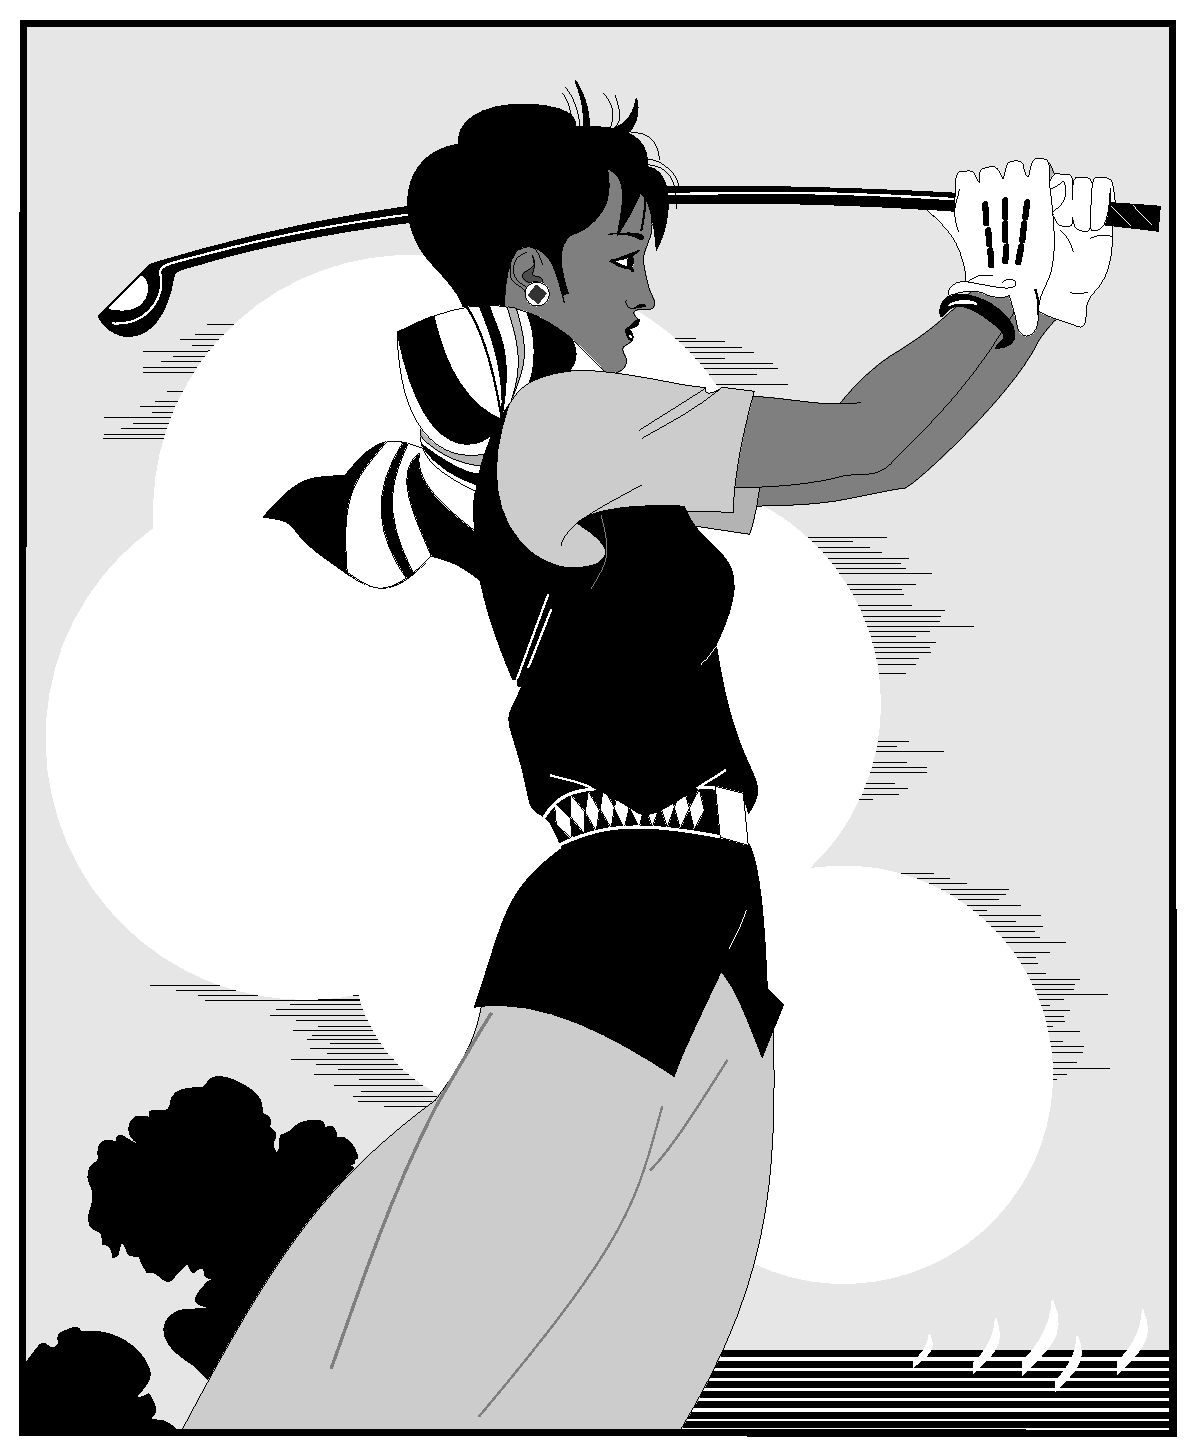
\includegraphics[width = 0.4\textwidth]{golfer}
\bicaption[golfer1]{}{打高尔夫球球的人(博士论文双语题注)}{Fig.$\!$}{The person playing golf (Doctoral thesis)}
\end{figure}

每个图均应有图题(由图序和图名组成),图题不宜有标点符号,图名在图序之后空1个半
角字符排写。图序按章编排,如第1章第一个插图的图号为“图1-1”。图题置于图下,硕士论
文只用中文,博士论文用中、英两种文字,居中书写,中文在上,要求中文用宋体5号字,
英文用Times New Roman 5号字。有图注或其它说明时应置于图题之上。引用图应注明出处
,在图题右上角加引用文献号。图中若有分图时,分图题置于分图之下或图题之下,可以只
用中文书写,分图号用a)、b)等表示。图中各部分说明应采用中文(引用的外文图除外)或
数字符号,各项文字说明置于图题之上(有分图时,置于分图题之上)。图中文字用宋体、
Times New Roman字体,字号尽量采用5号字(当字数较多时可用小5号字,以清晰表达为原
则,但在一个插图内字号要统一)。同一图内使用文字应统一。图表中物理量、符号用斜体
。
\subsection{本硕论文题注}[Other picture example]

本硕论文题注如\figref{fig:bm}所示。

\begin{figure}[ht]
\centering
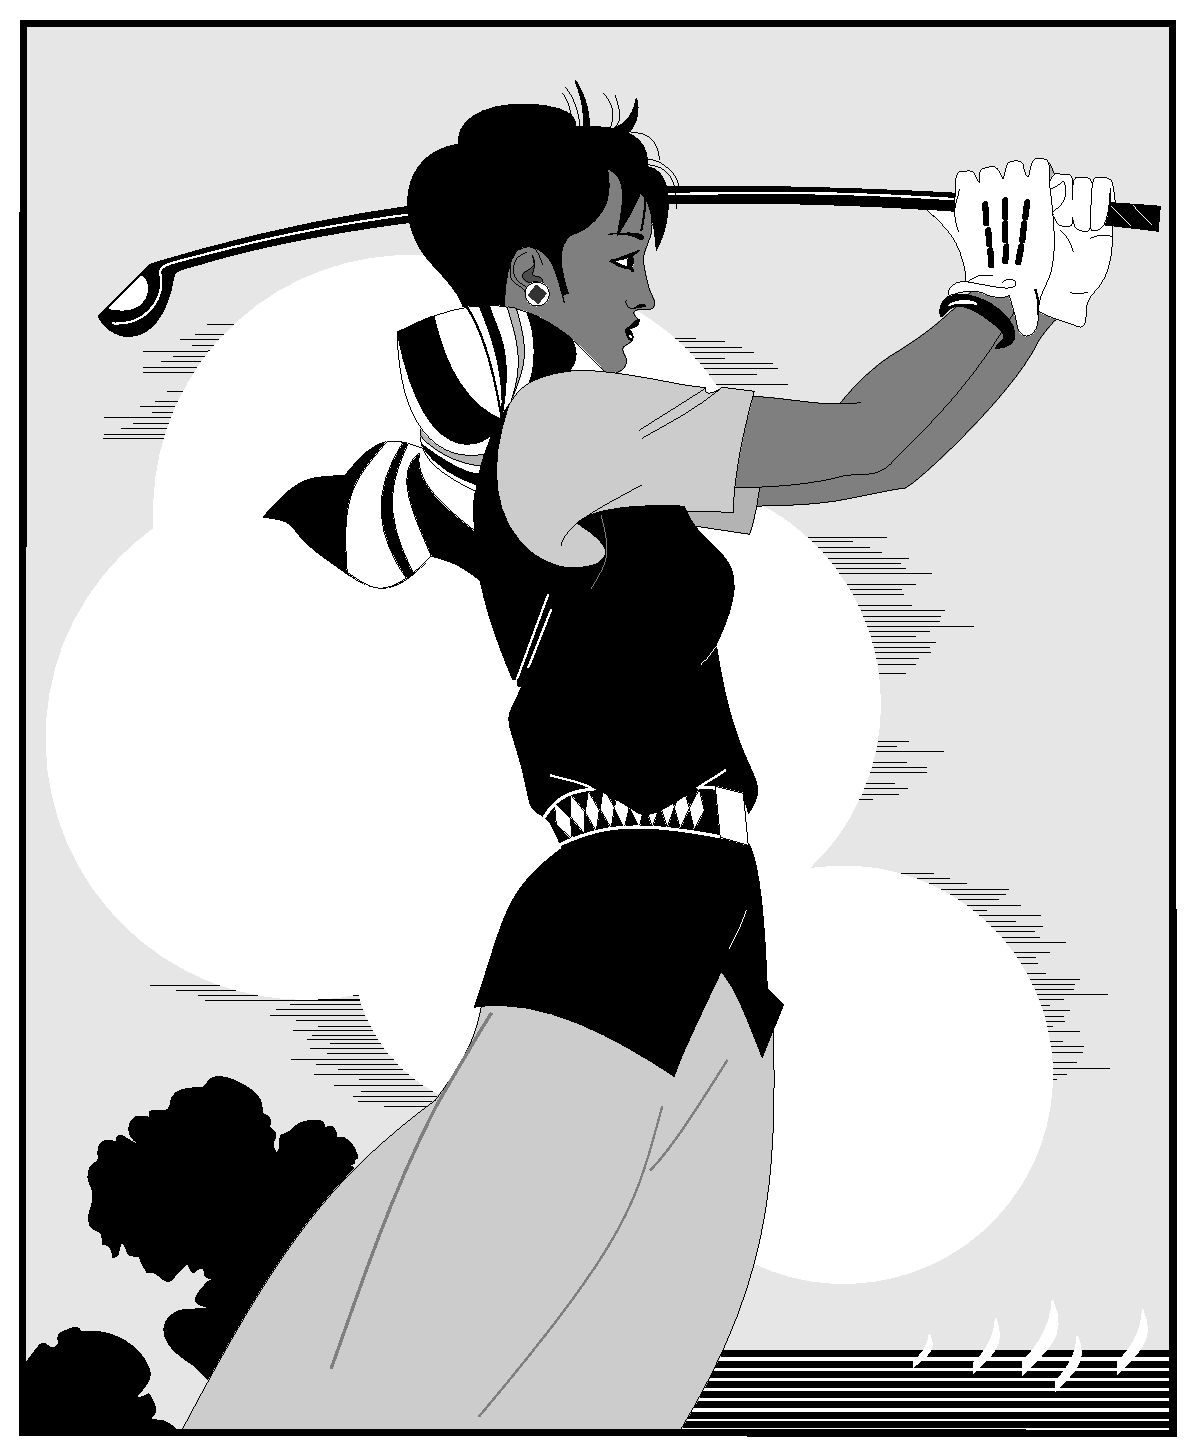
\includegraphics[width = 0.4\textwidth]{golfer}
\caption{打高尔夫球的人,硕士论文要求只用汉语}
\label{fig:bm}
\end{figure}

\subsection{并排图和子图}[Abreast-picture and Sub-picture example]
\subsubsection{并排图}[Abreast-picture example]

使用并排图时,需要注意对齐方式。默认情况是中部对齐。这里给出中部对齐、顶部对齐
、图片底部对齐三种常见方式。其中,底部对齐方式有一个很巧妙的方式,将长度比较小
的图放在左面即可。

\lipsum[2]

\begin{figure}[htbp]
\centering
\begin{minipage}{0.4\textwidth}
\centering
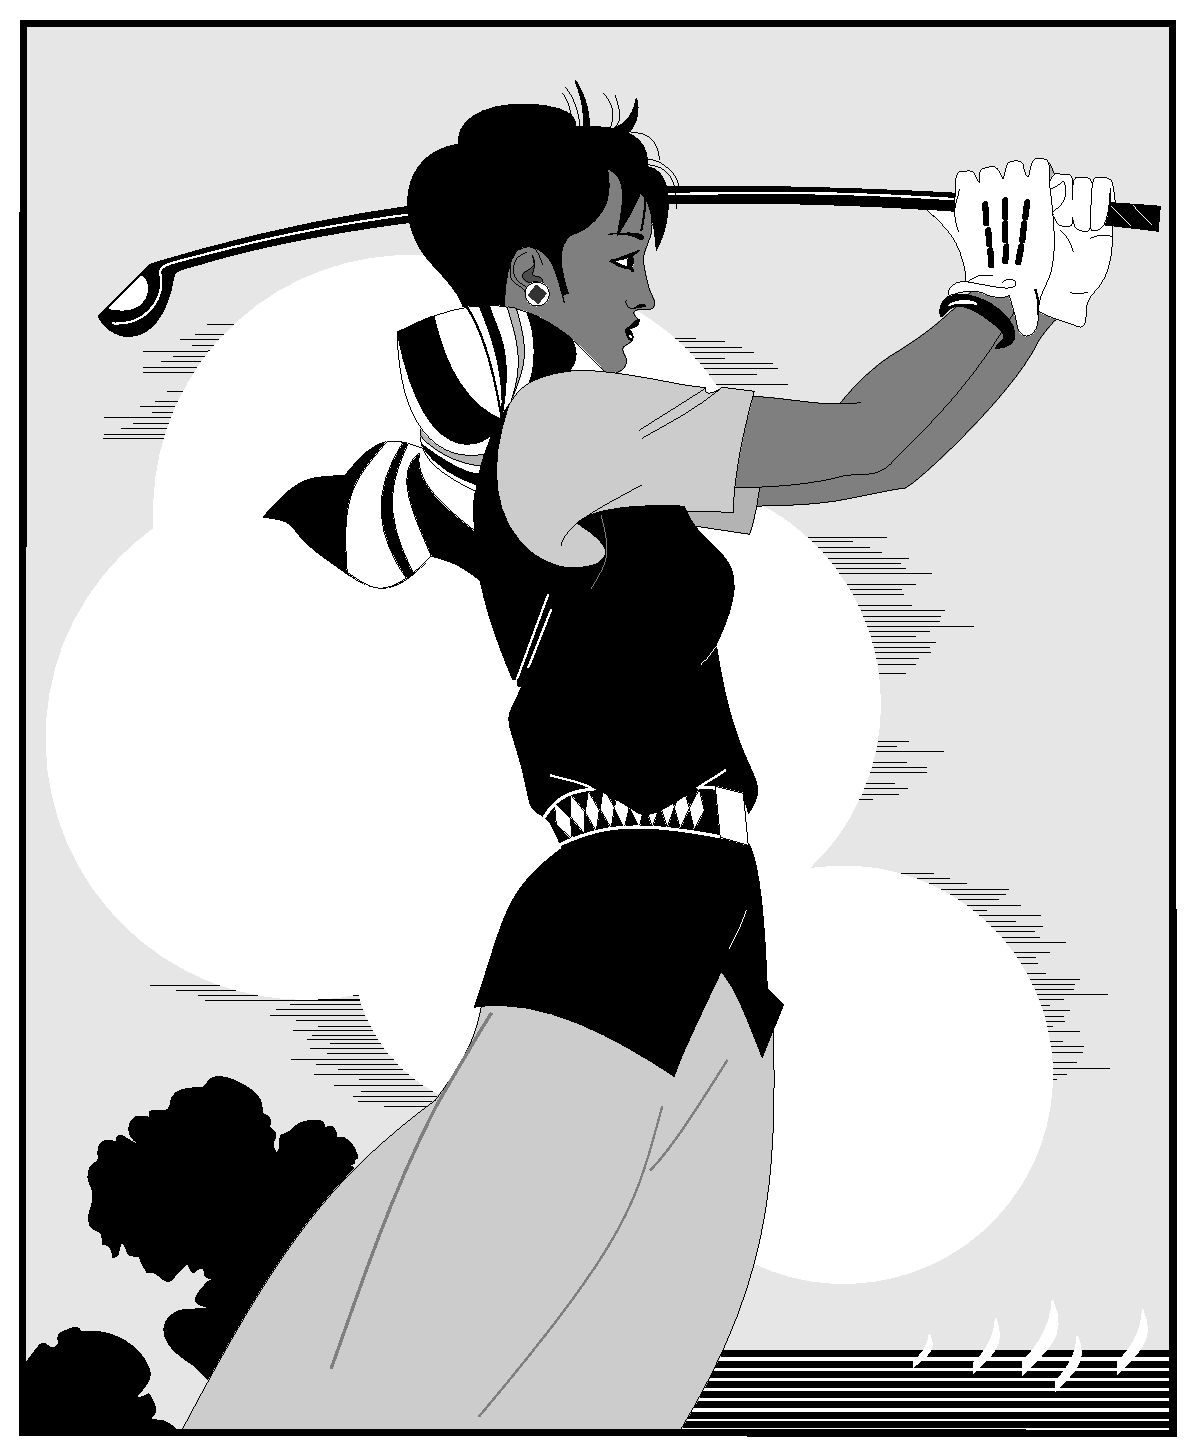
\includegraphics[width=\textwidth]{golfer}
\bicaption[golfer2]{}{打高尔夫球的人}{Fig.$\!$}{The person playing golf}
\end{minipage}
\centering
\begin{minipage}{0.4\textwidth}
\centering
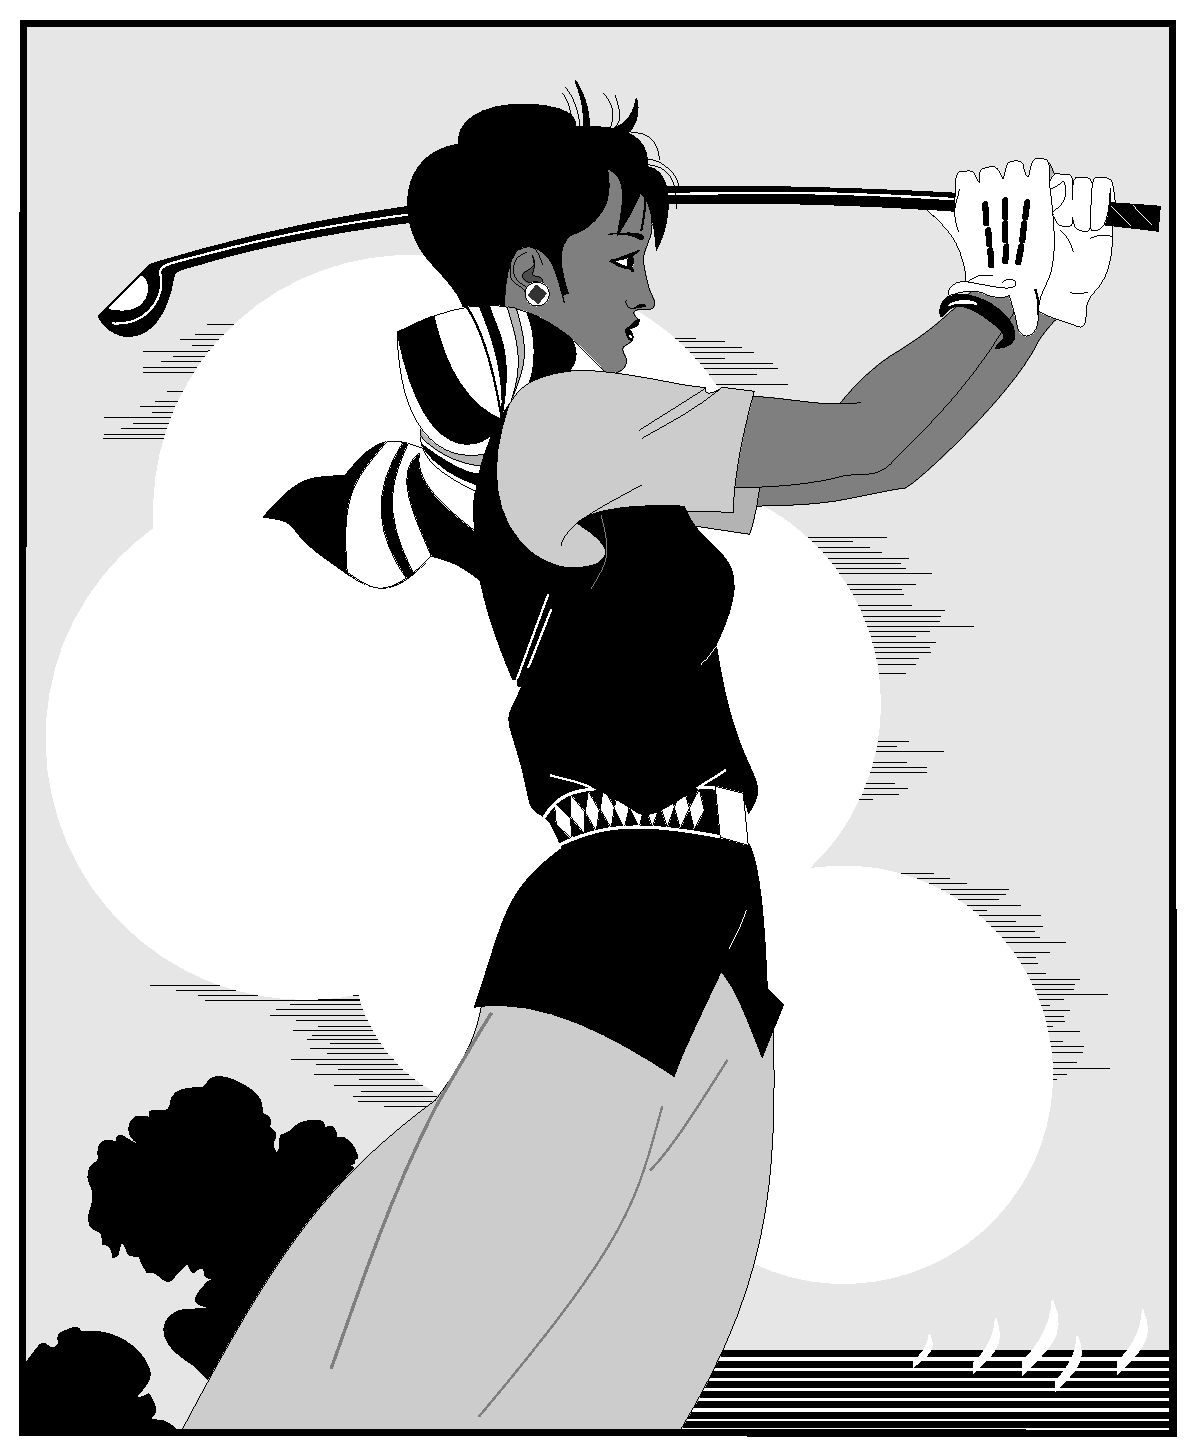
\includegraphics[width=\textwidth]{golfer}
\bicaption[golfer3]{}{打高尔夫球的人。注意,这里默认居中}{Fig.$\!$}{The person playing golf. Please note that, it is vertically center aligned by default.}
\end{minipage}
\end{figure}

\begin{figure}[htbp]
\centering
\begin{minipage}[t]{0.4\textwidth}
\centering
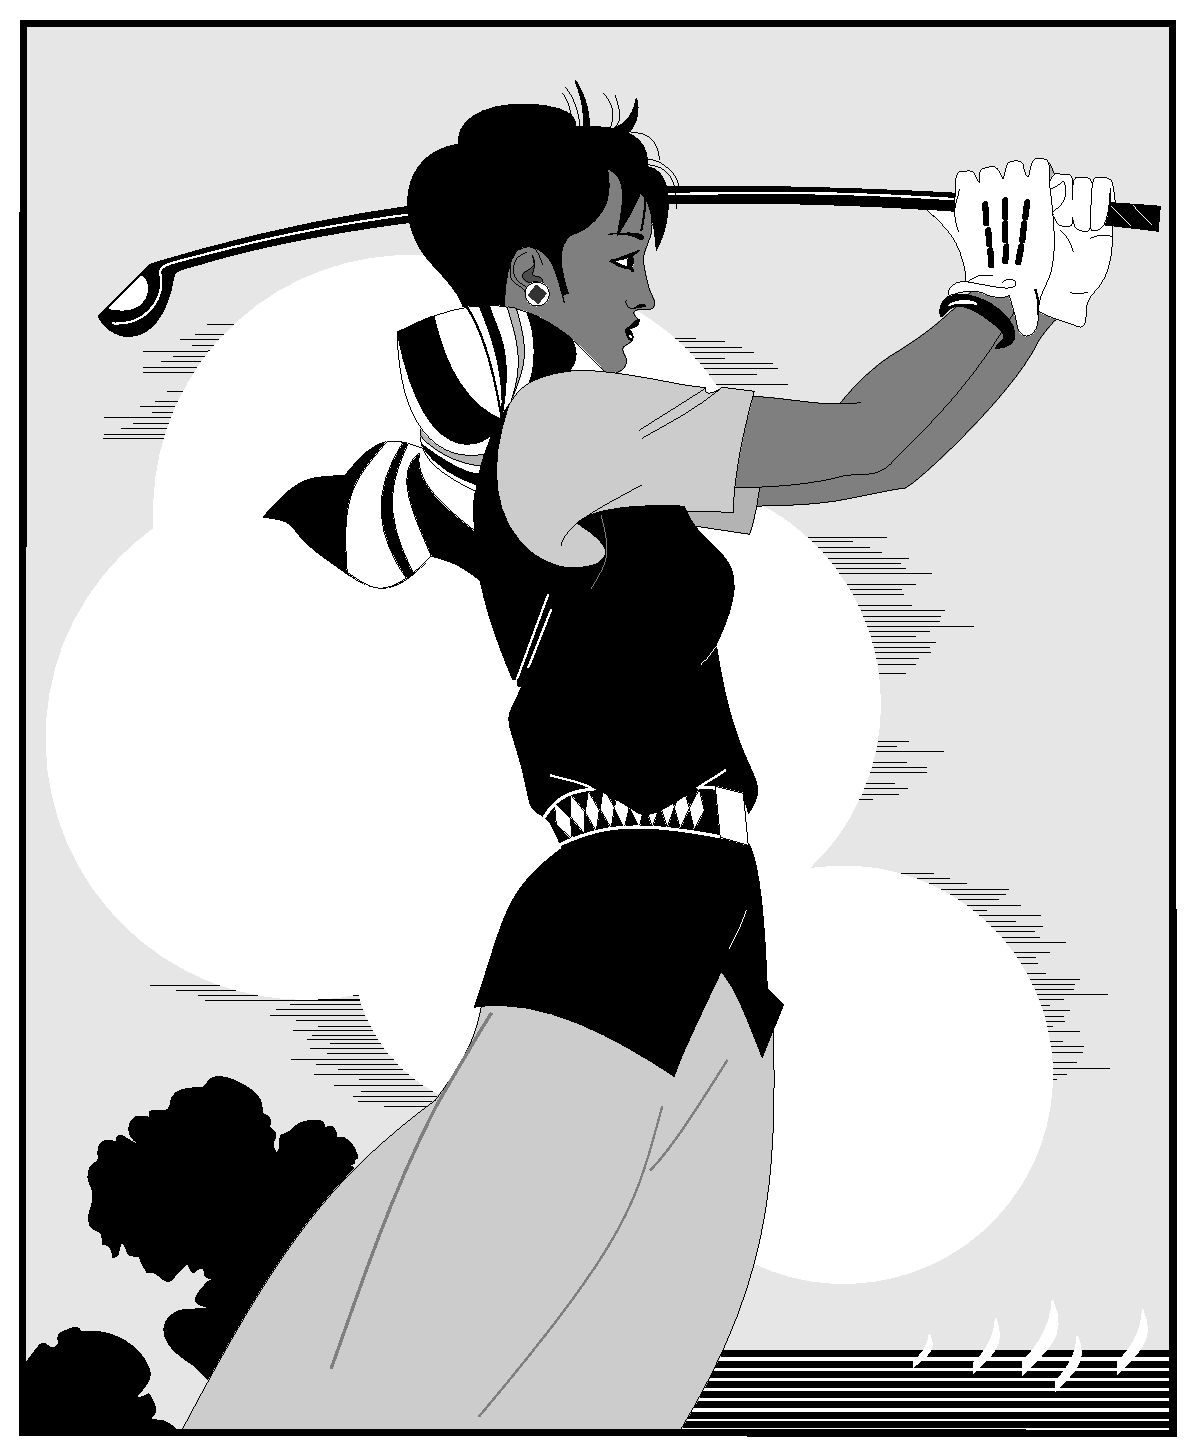
\includegraphics[width=\textwidth]{golfer}
\bicaption[golfer5]{}{打高尔夫球的人}{Fig.$\!$}{The person playing golf}
\end{minipage}
\centering
\begin{minipage}[t]{0.4\textwidth}
\centering
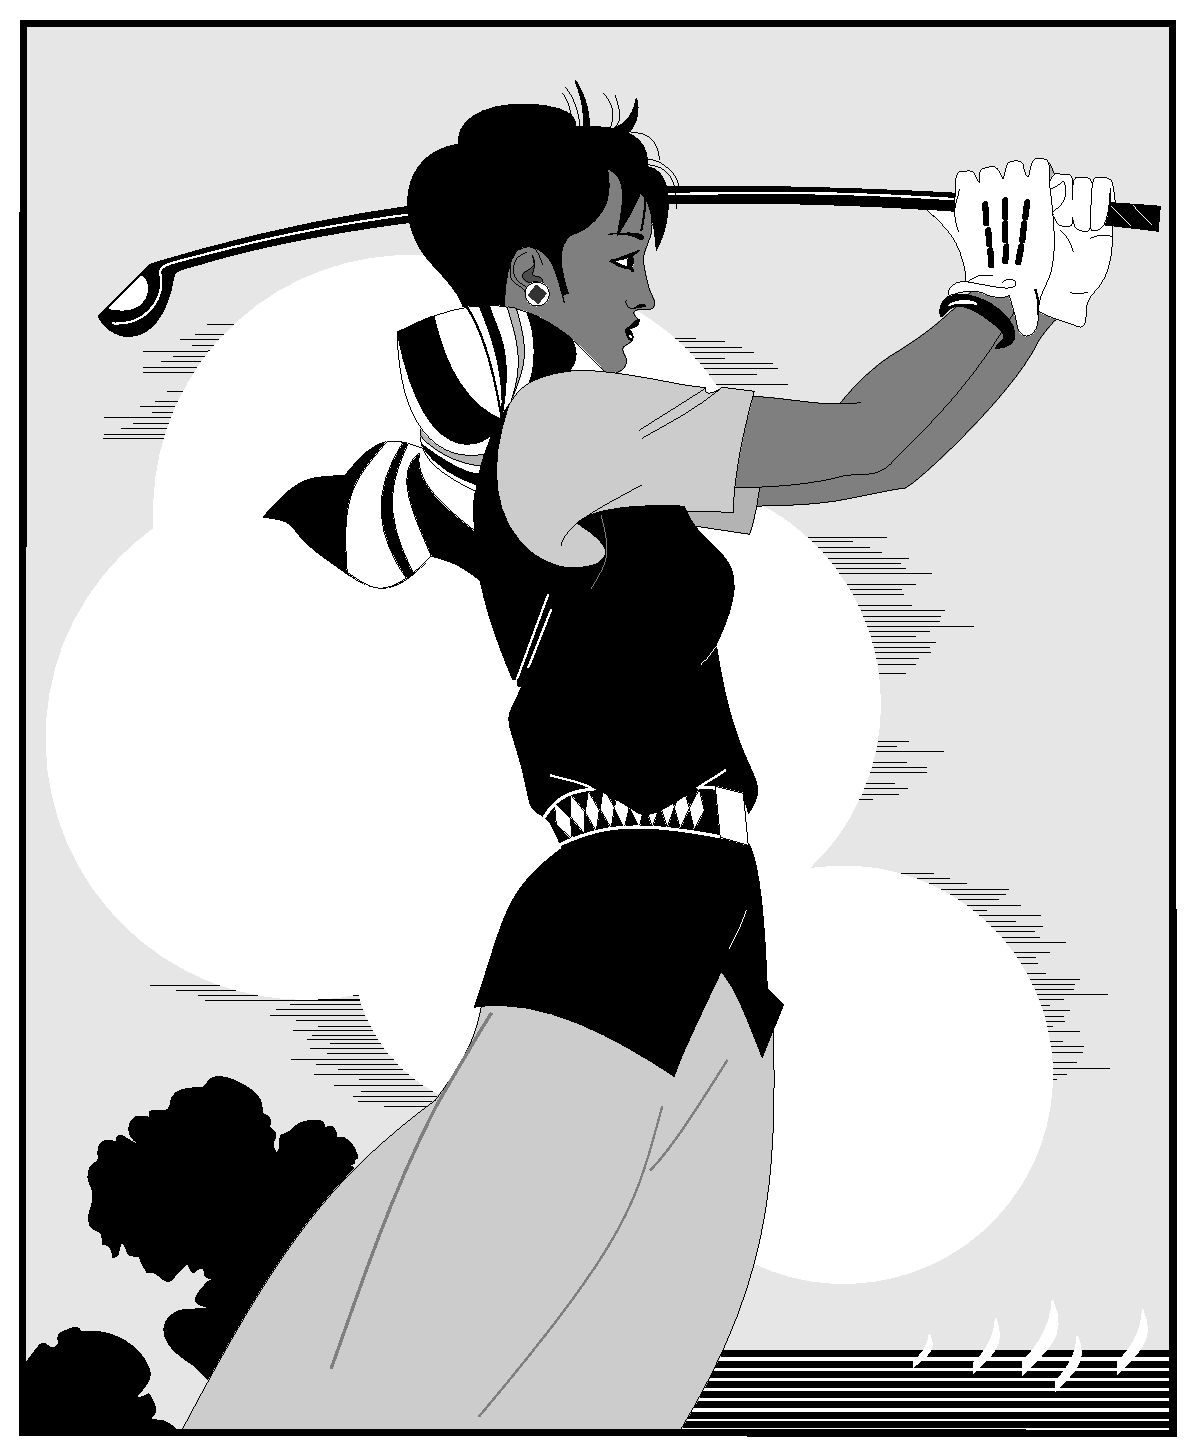
\includegraphics[width=\textwidth]{golfer}
\bicaption[golfer8]{}{打高尔夫球的人。注意,此图是顶部对齐}{Fig.$\!$}{The person playing golf. Please note that, it is vertically top aligned.}
\end{minipage}
\end{figure}

\begin{figure}[htbp]
\centering
\begin{minipage}[t]{0.4\textwidth}
\centering
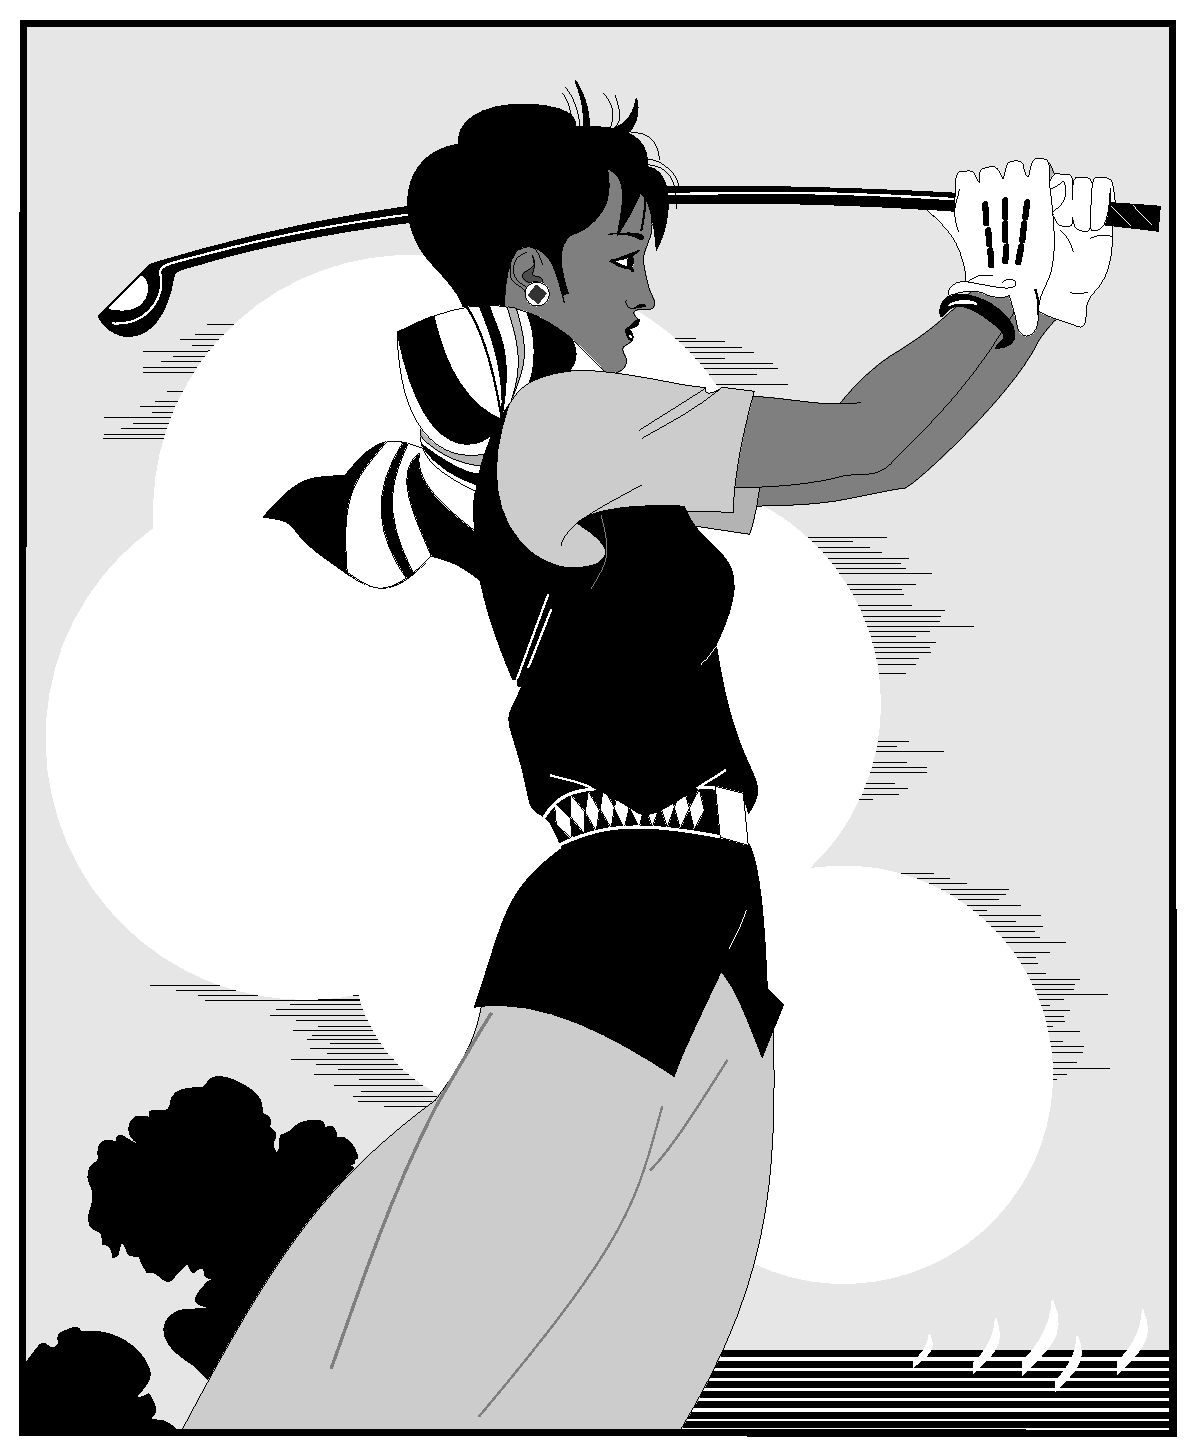
\includegraphics[width=\textwidth,height=\textwidth]{golfer}
\bicaption[golfer9]{}{打高尔夫球的人。注意,此图对齐方式是图片底部对齐}{Fig.$\!$}{The person playing golf. Please note that, it is vertically bottom aligned for figure.}
\end{minipage}
\centering
\begin{minipage}[t]{0.4\textwidth}
\centering
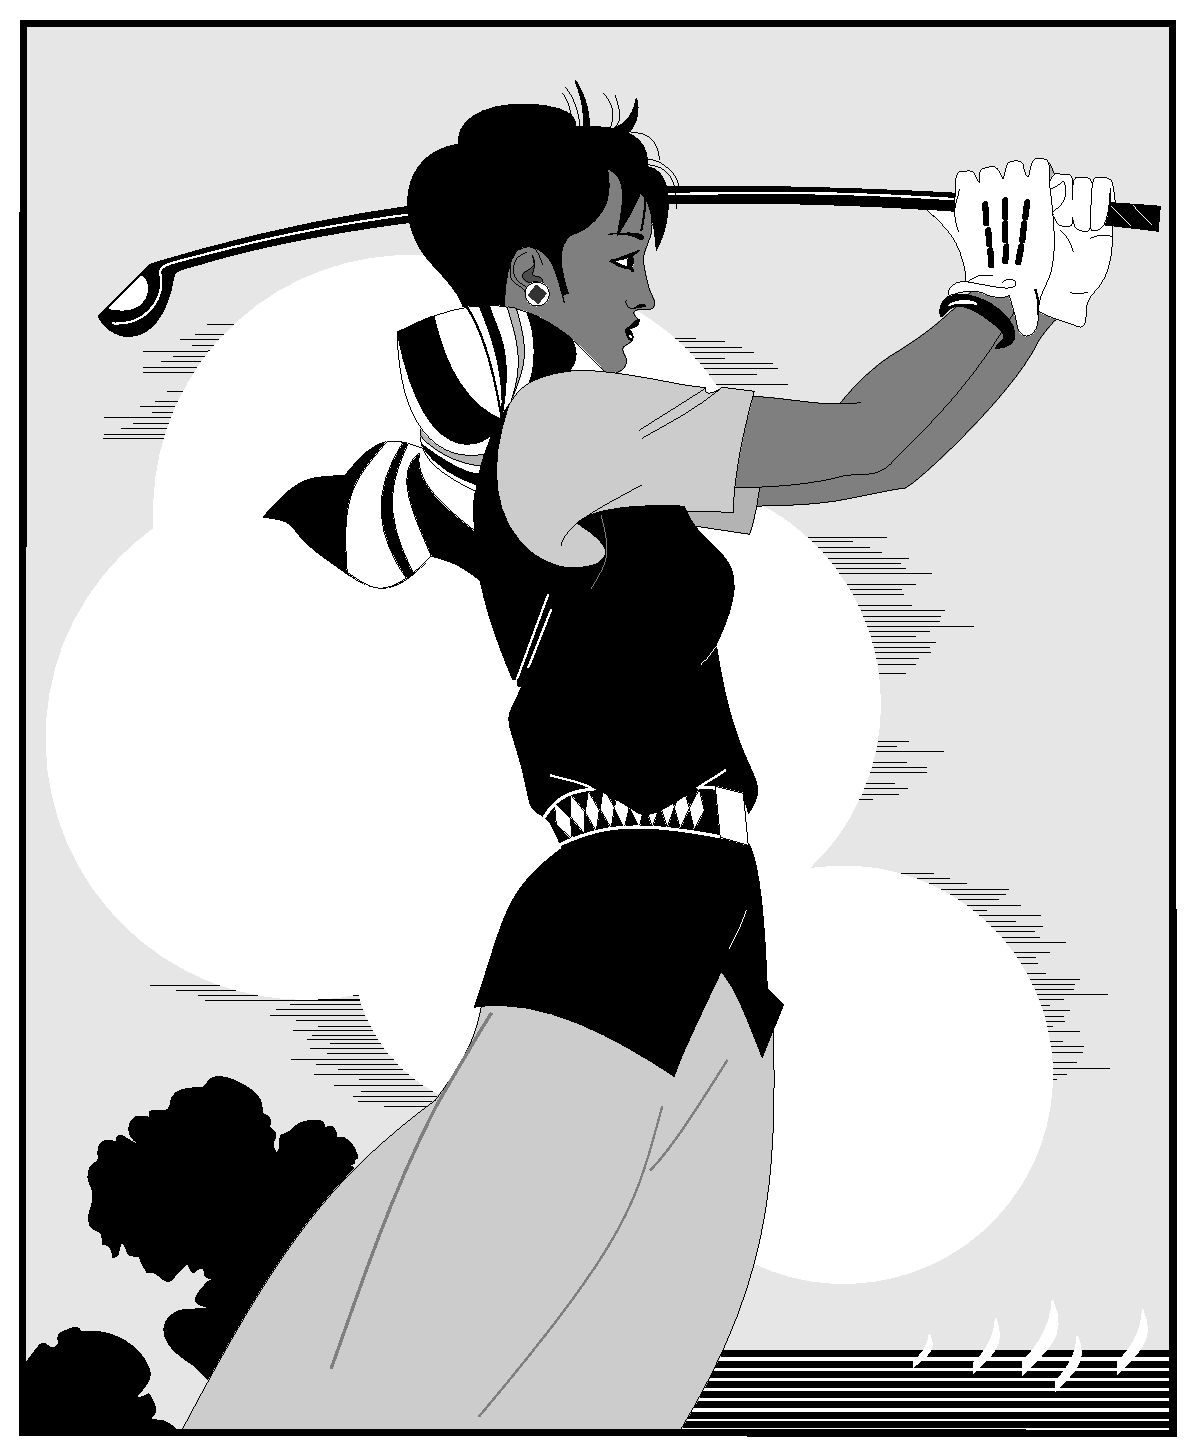
\includegraphics[width=\textwidth]{golfer}
\bicaption[golfer6]{}{打高尔夫球的人}{Fig.$\!$}{The person playing golf}
\end{minipage}
\end{figure}

\subsubsection{子图}[Sub-picture example]

注意:子图题注也可以只用中文。规范规定“分图题置于分图之下或图题之下”,但没有给出具体的格式要求。
没有要求的另外一个说法就是“无论什么格式都不对”。
所以只有在一个图中有标注“(a),(b)”,无法使用\cs{subfigure}的情况下,使用最后一个图例中的格式设置方法,否则不要使用。
为了应对“无论什么格式都不对”,这个子图图题使用“minipage”和“description”环境,宽度,对齐方式可以按照个人喜好自由设置,是否使用双语子图图题也可以自由设置。

\lipsum[1-3]

无意义文字,每页底部不要留空白。

\lipsum[4-5]

\begin{figure}[!ht]
\setlength{\subfigcapskip}{-1bp}
\centering
\begin{minipage}{\textwidth}
\centering
\subfigure{\label{golfer41}}\addtocounter{subfigure}{-2}
\subfigure[The person playing golf]{\subfigure[打高尔夫球的人~1]{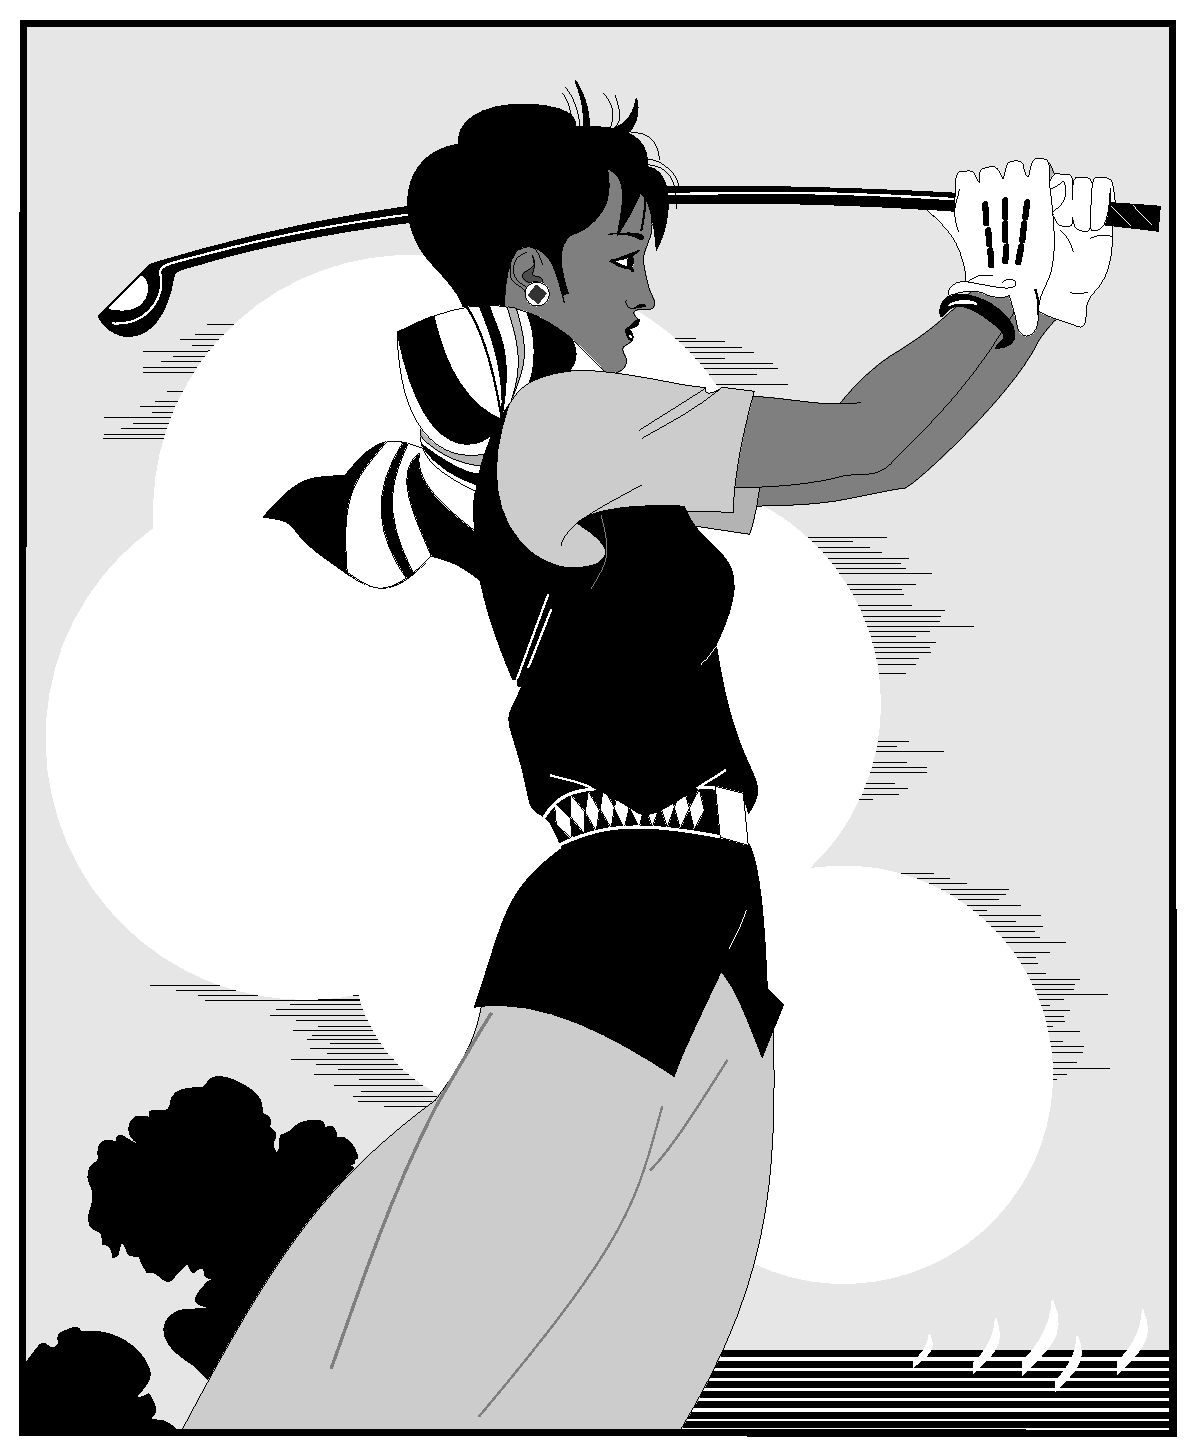
\includegraphics[width=0.4\textwidth]{golfer}}}
\hspace{2em}
\subfigure{\label{golfer42}}\addtocounter{subfigure}{-2}
\subfigure[The person playing golf]{\subfigure[打高尔夫球的人~2]{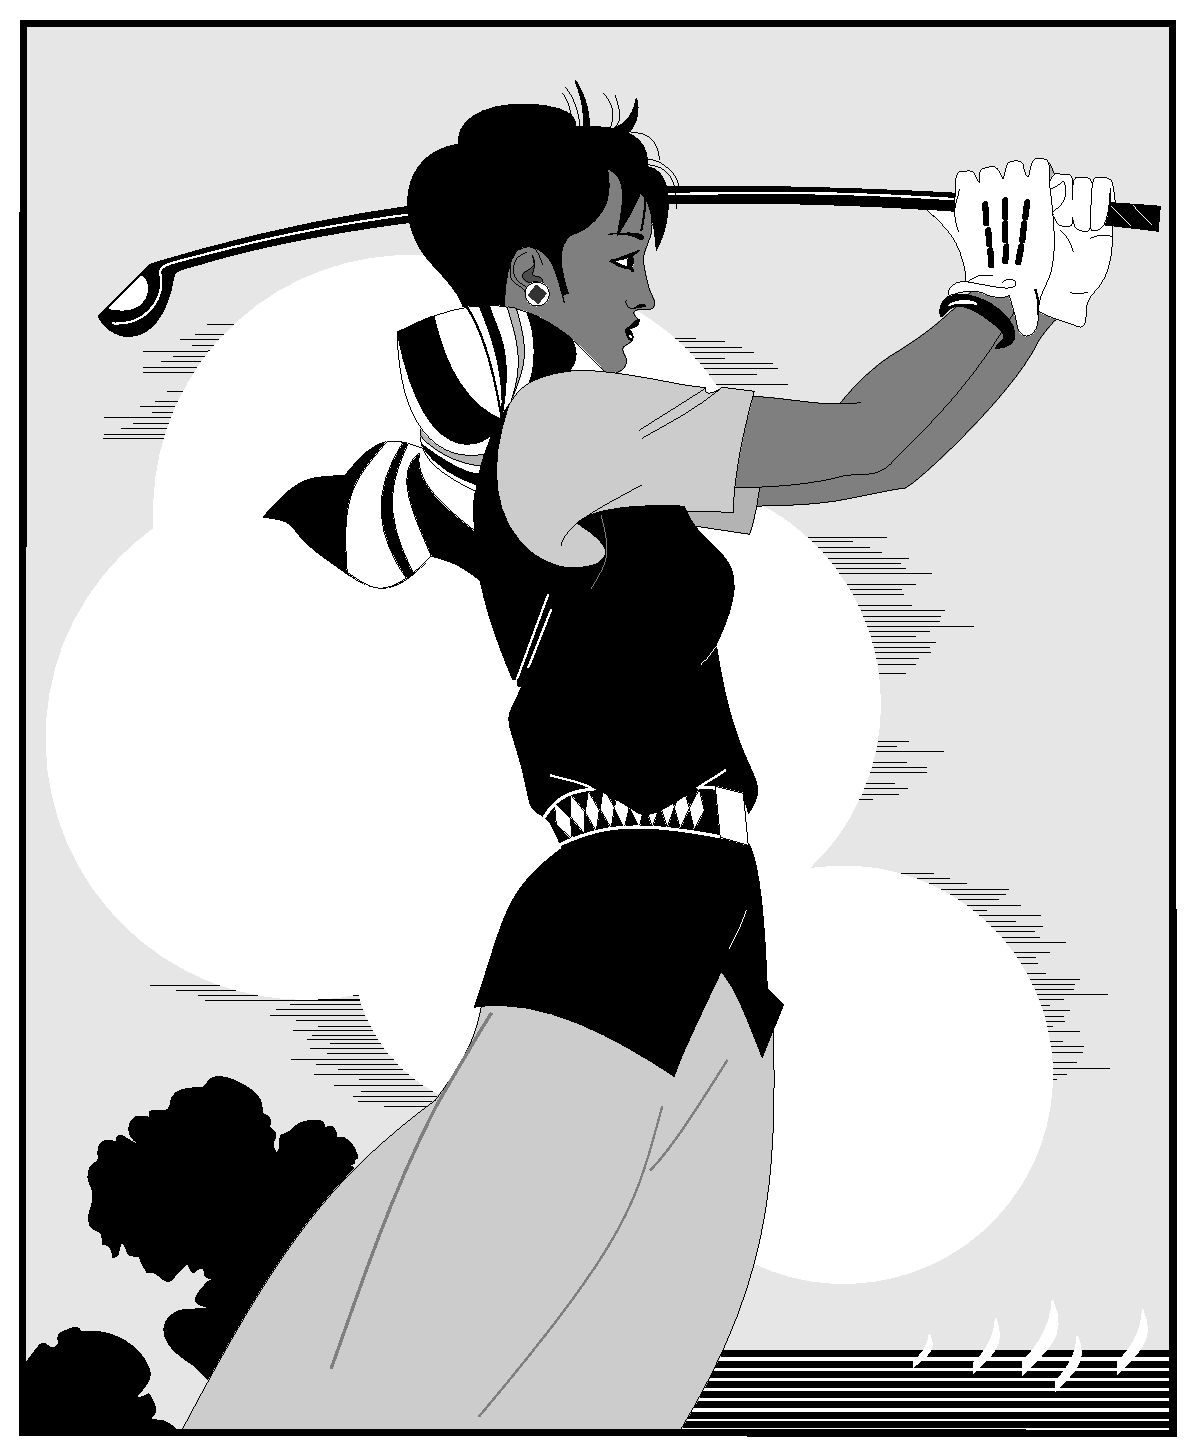
\includegraphics[width=0.4\textwidth]{golfer}}}
\end{minipage}
\centering
\begin{minipage}{\textwidth}
\centering
\subfigure{\label{golfer43}}\addtocounter{subfigure}{-2}
\subfigure[The person playing golf]{\subfigure[打高尔夫球的人~3]{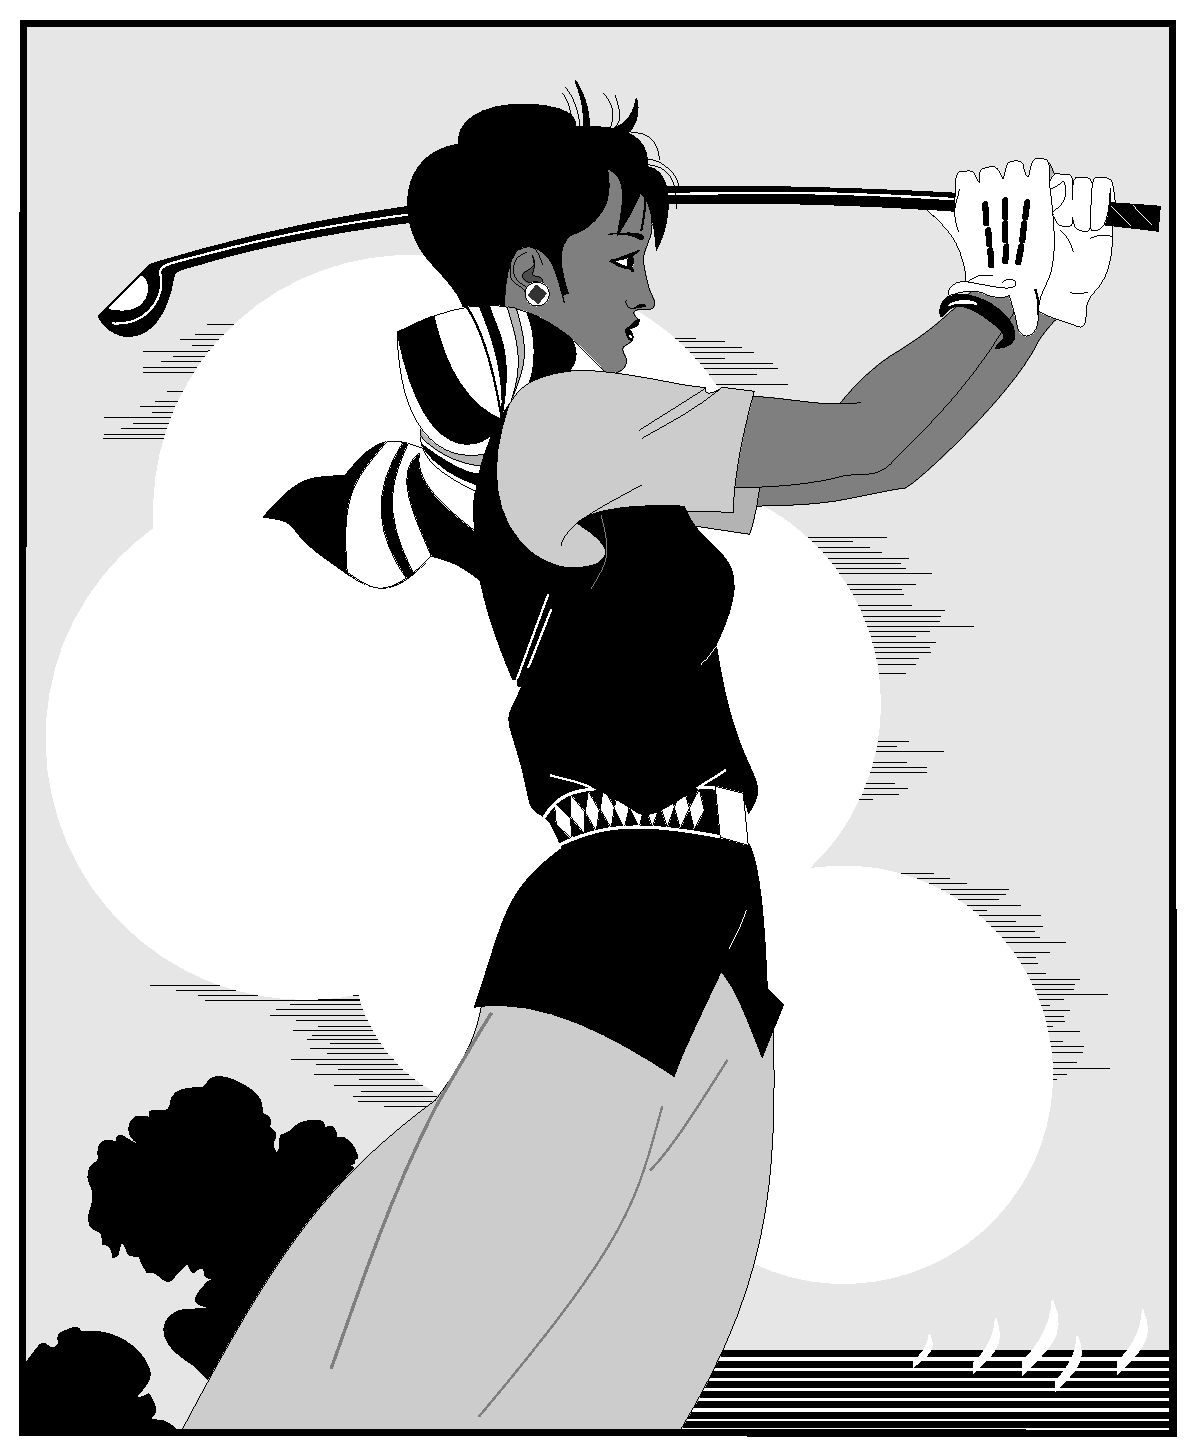
\includegraphics[width=0.4\textwidth]{golfer}}}
\hspace{2em}
\subfigure{\label{golfer44}}\addtocounter{subfigure}{-2}
\subfigure[The person playing golf. Here, 'hang indent' and 'center last line' are not stipulated in the regulation.]{\subfigure[打高尔夫球的人~4。注意,规范中没有明确规定要悬挂缩进、最后一行居中。]{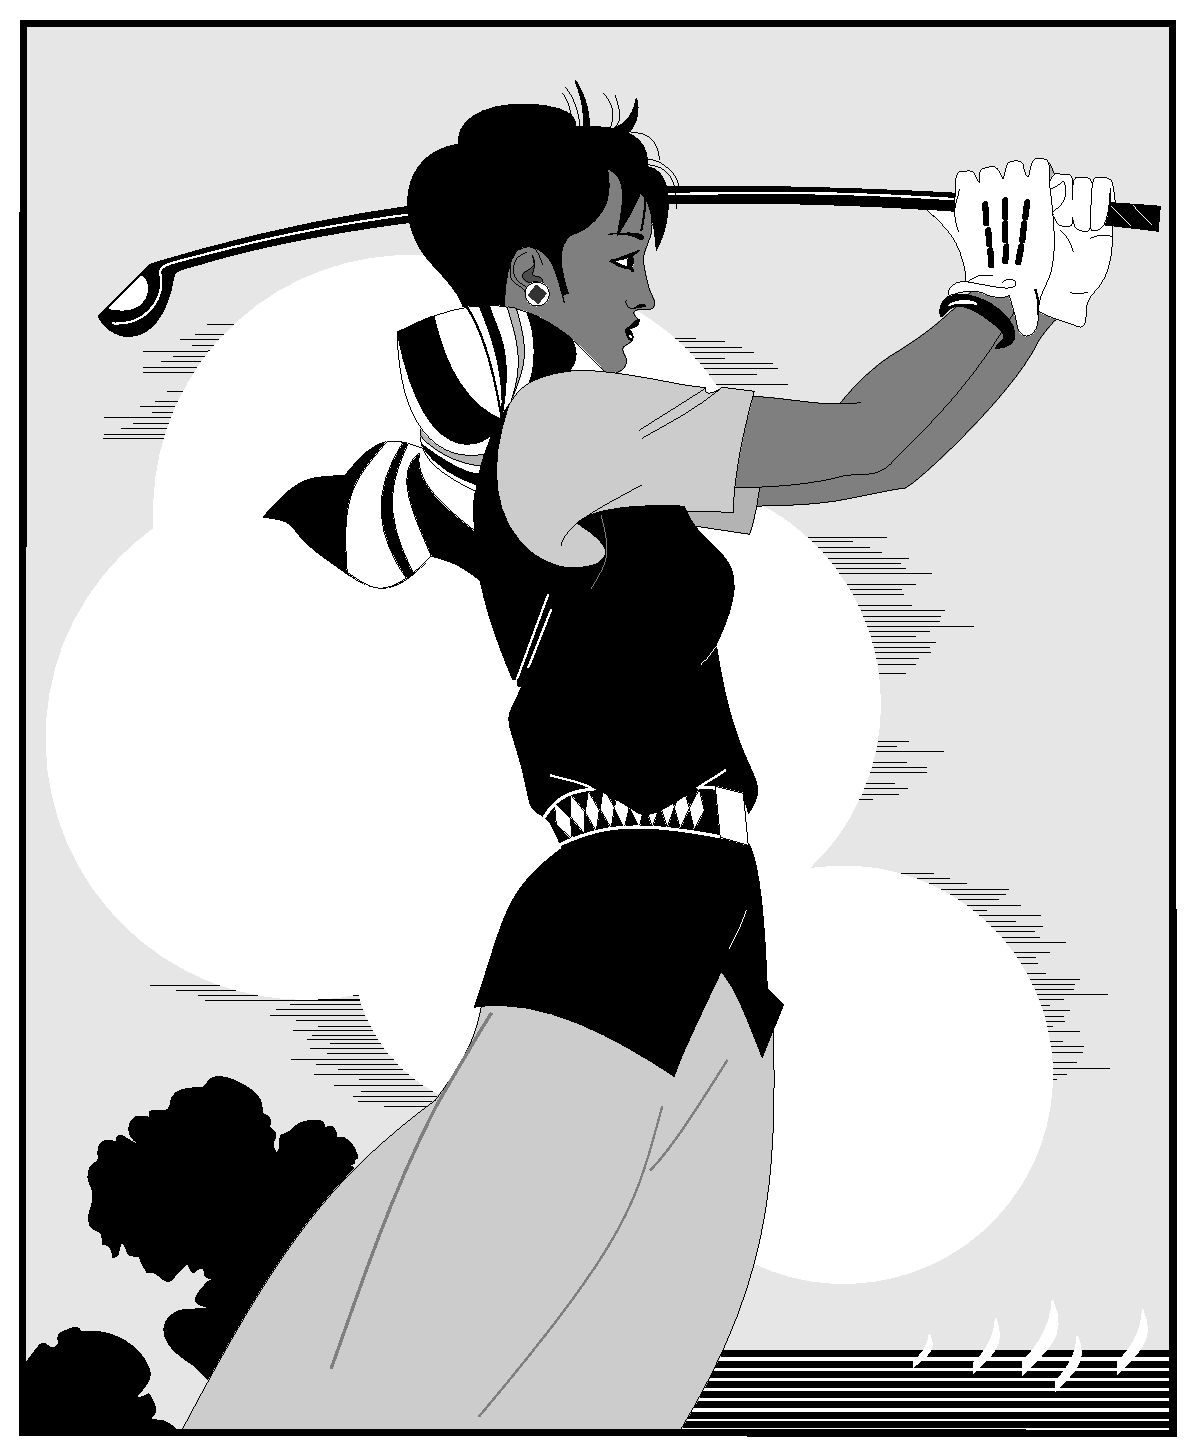
\includegraphics[width=0.4\textwidth]{golfer}}}
\end{minipage}
\vspace{0.2em}
\bicaption[golfer4]{}{打高尔夫球的人}{Fig.$\!$}{The person playing gol}
\end{figure}

\begin{figure}[t]
  \centering
  \begin{minipage}{.7\linewidth}
    \setlength{\subfigcapskip}{-1bp}
    \centering
    \begin{minipage}{\textwidth}
      \centering
      \subfigure{\label{golfer45}}\addtocounter{subfigure}{-2}
      \subfigure[The person playing golf]{\subfigure[打高尔夫球的人~1]{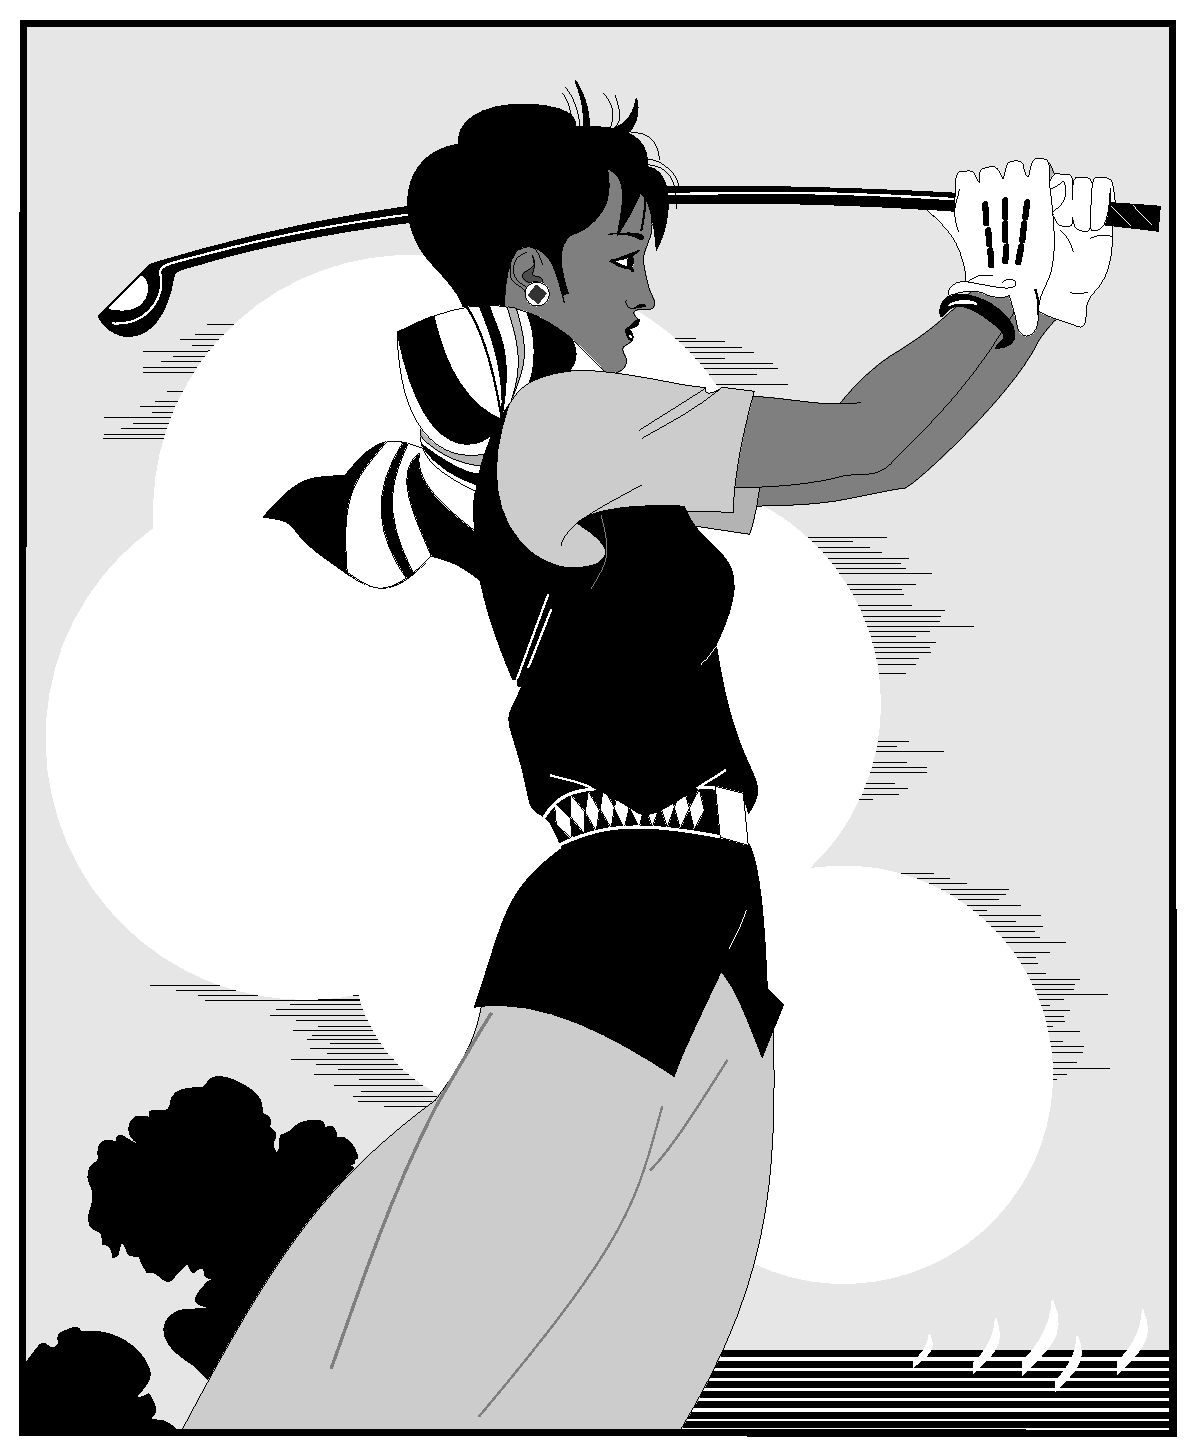
\includegraphics[width=0.4\textwidth]{golfer}}}
      \hspace{4em}
      \subfigure{\label{golfer46}}\addtocounter{subfigure}{-2}
      \subfigure[The person playing golf]{\subfigure[打高尔夫球的人~2]{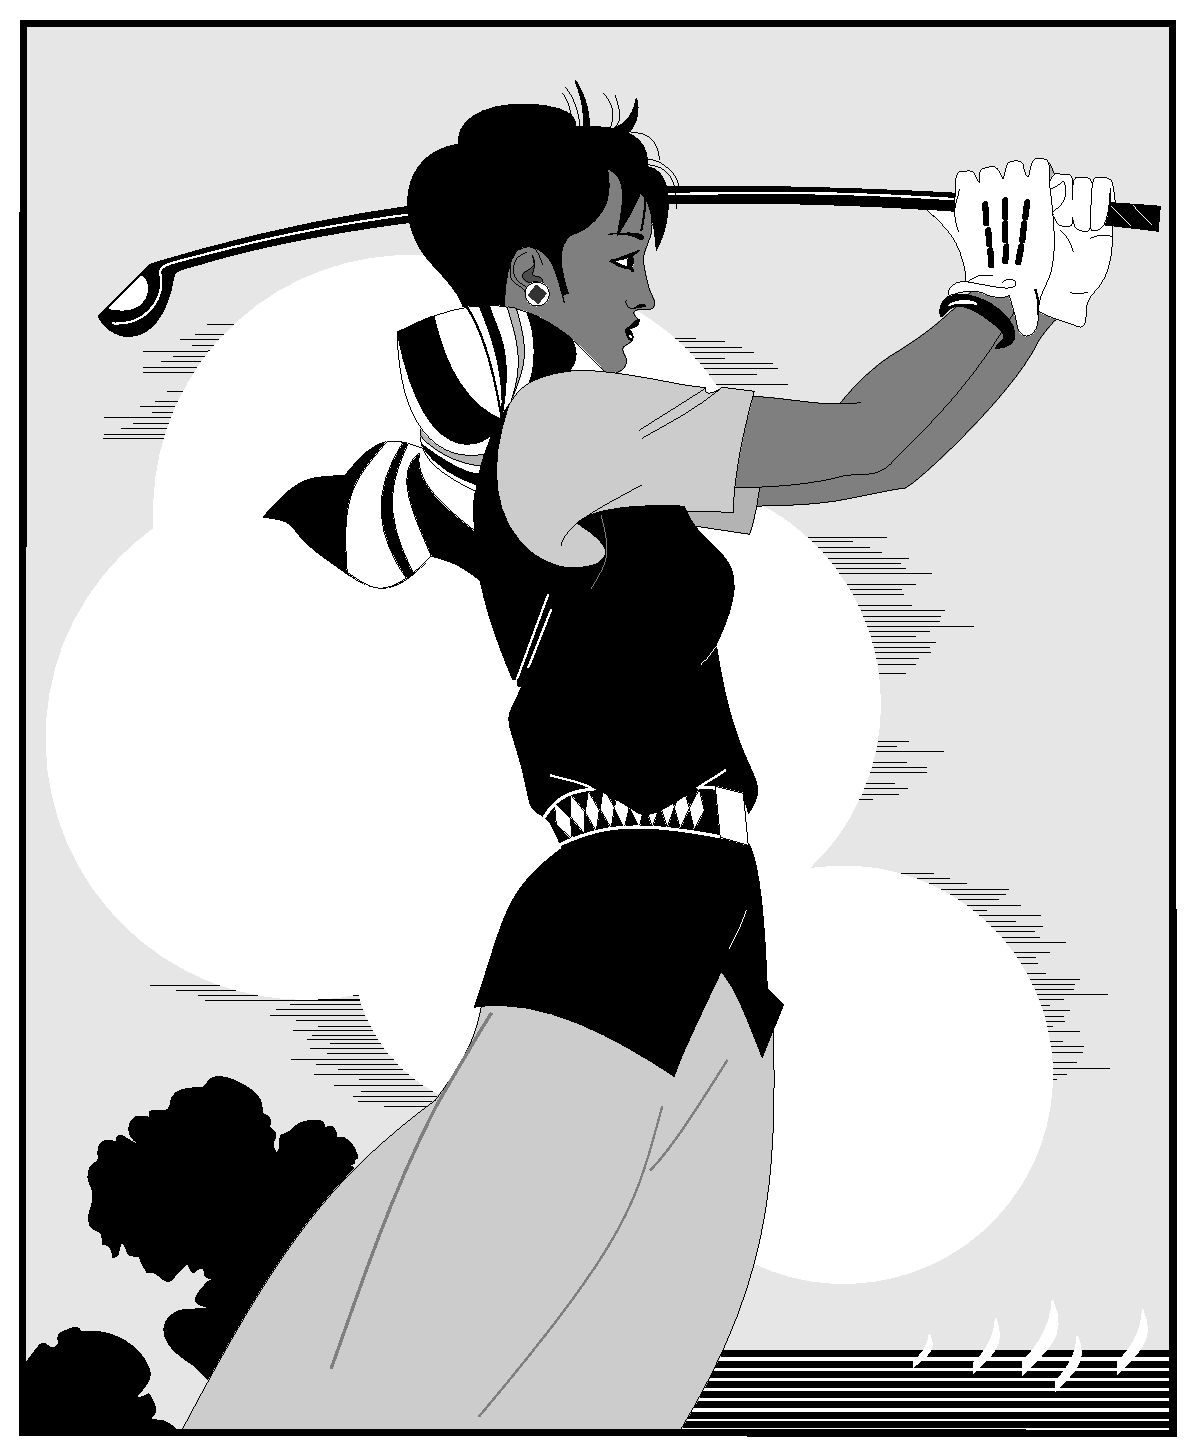
\includegraphics[width=0.4\textwidth]{golfer}}}
    \end{minipage}
    \vskip 0.2em
  \wuhao 注意:这里是中文图注添加位置(我工要求,图注在图题之上)。
    \vspace{0.2em}
\bicaption[golfer47]{}{打高尔夫球的人。注意,此处我工有另外一处要求,子图图题可以位于主图题之下。但由于没有明确说明位于下方具体是什么格式,所以这里不给出举例。}{Fig.$\!$}{The person playing golf. Please note that, although it is appropriate to put subfigures' captions under this caption as stipulated in regulation, but its format is not clearly stated.}
  \end{minipage}
\end{figure}

\begin{figure}[t]
\centering
% \begin{tikzpicture}
% 	\node[anchor=south west,inner sep=0] (image) at (0,0) {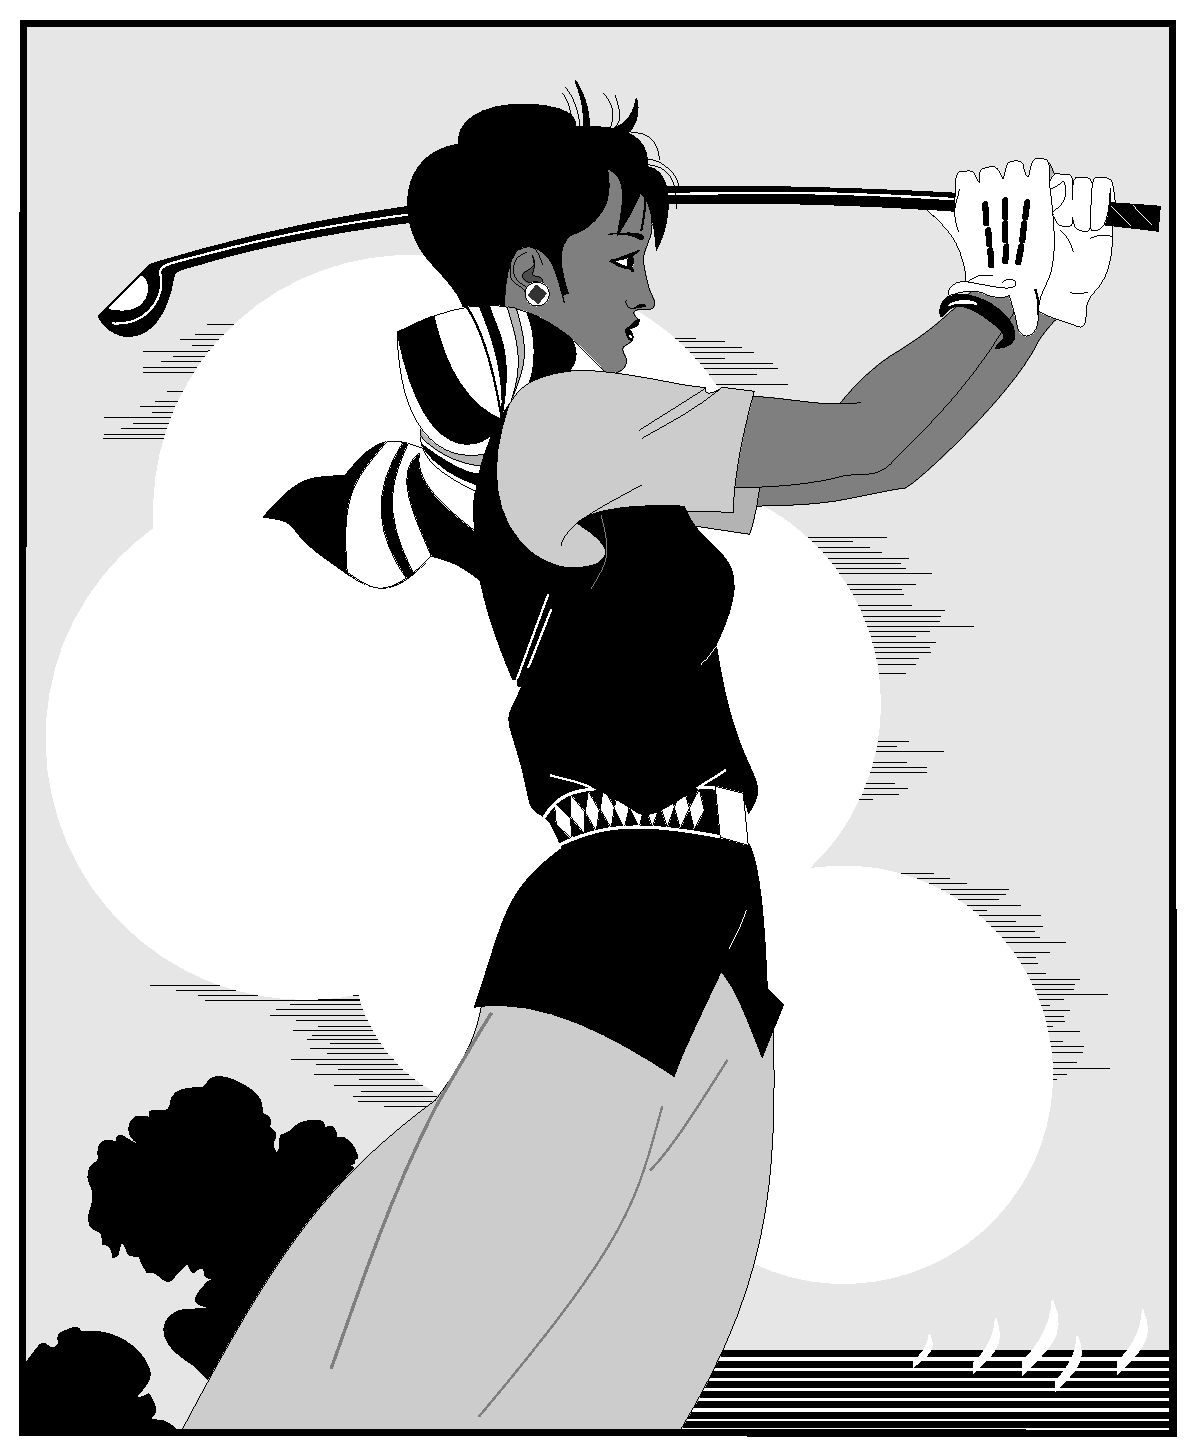
\includegraphics[width=0.3\textwidth]{golfer}};
% 	\begin{scope}[x={(image.south east)},y={(image.north west)}]
% 		\node at (0.3,0.5) {a)};
% 		\node at (0.8,0.2) {b)};
% 	\end{scope}
% \end{tikzpicture}
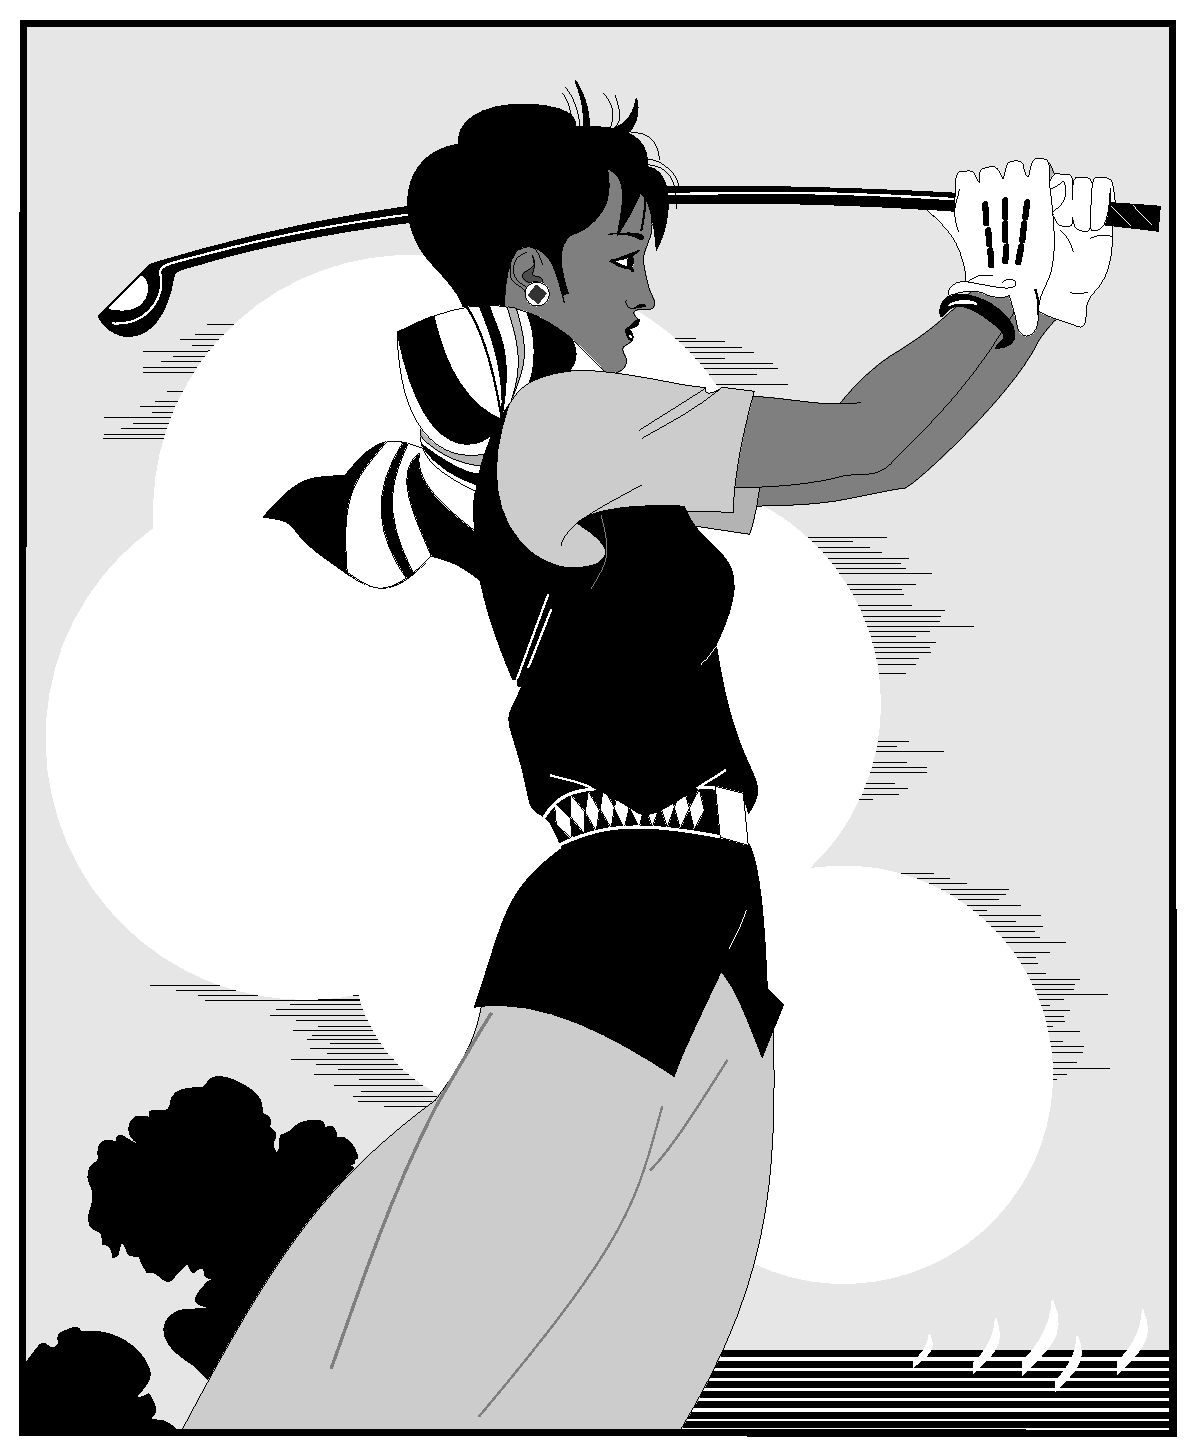
\includegraphics[width=0.3\textwidth]{golfer}
\bicaption[golfer0]{}{打高尔夫球球的人(博士论文双语题注)}{Fig.$\!$}{The person playing golf (Doctoral thesis)}
\vskip -0.4em
 \hspace{2em}
\begin{minipage}[t]{0.3\textwidth}
\wuhao \setlist[description]{font=\normalfont}
	\begin{description}
		\item[(a)]子图图题
		\item[(a)]Subfigure caption
	\end{description}
 \end{minipage}
 \hspace{2em}
 \begin{minipage}[t]{0.3\textwidth}
\wuhao \setlist[description]{font=\normalfont}
	\begin{description}
		\item[(b)]子图图题
		\item[(b)]Subfigure caption
	\end{description}
\end{minipage}
\end{figure}

\begin{figure}[!ht]
	\centering
	\begin{sideways}
		\begin{minipage}{\textheight}
			\centering
			\fbox{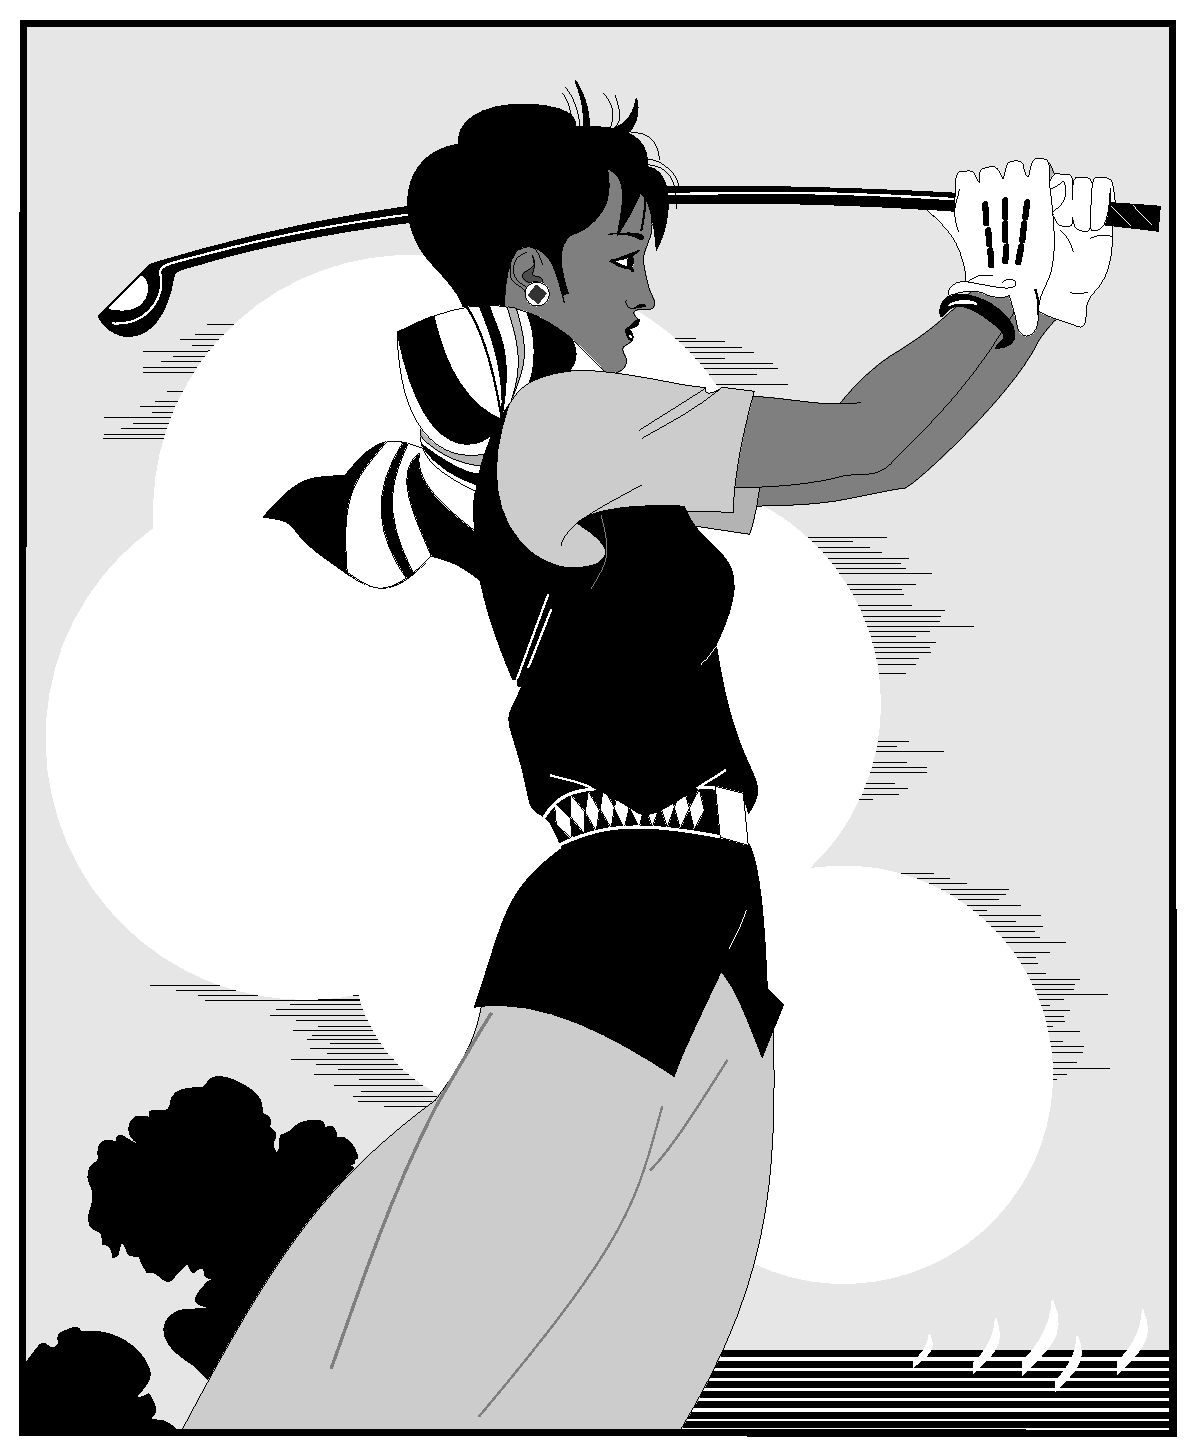
\includegraphics[width=0.2\textwidth]{golfer}}
			\fbox{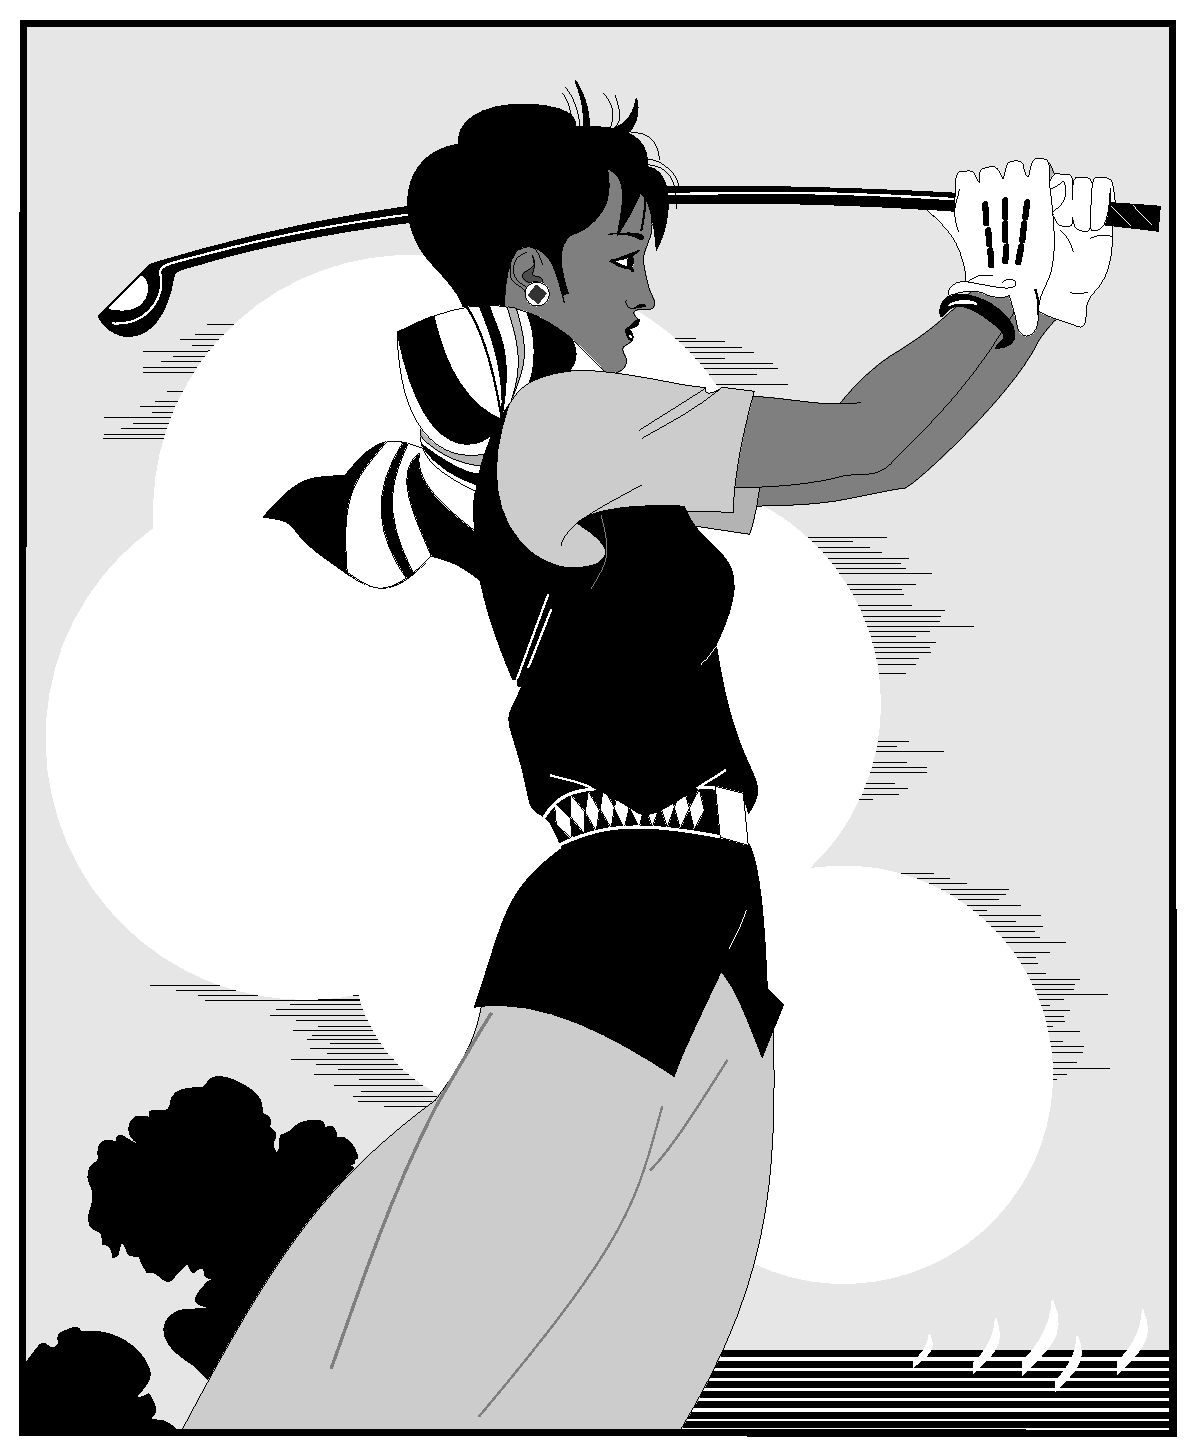
\includegraphics[width=0.2\textwidth]{golfer}}
			\fbox{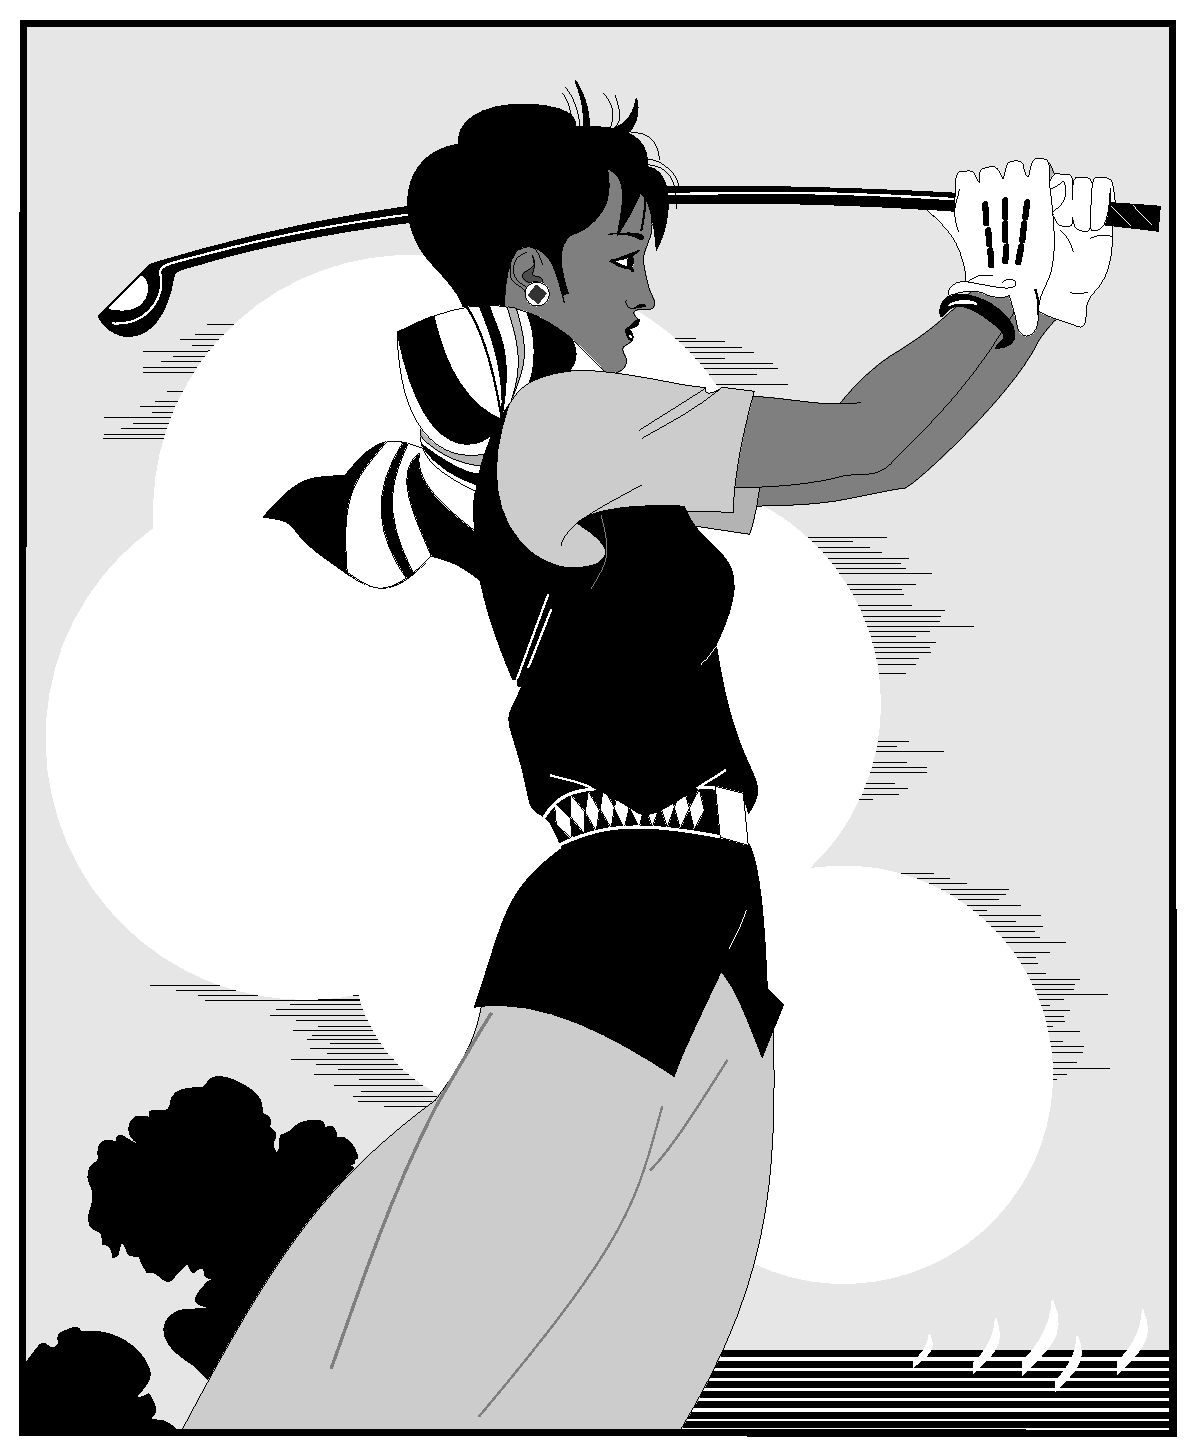
\includegraphics[width=0.2\textwidth]{golfer}}
			\fbox{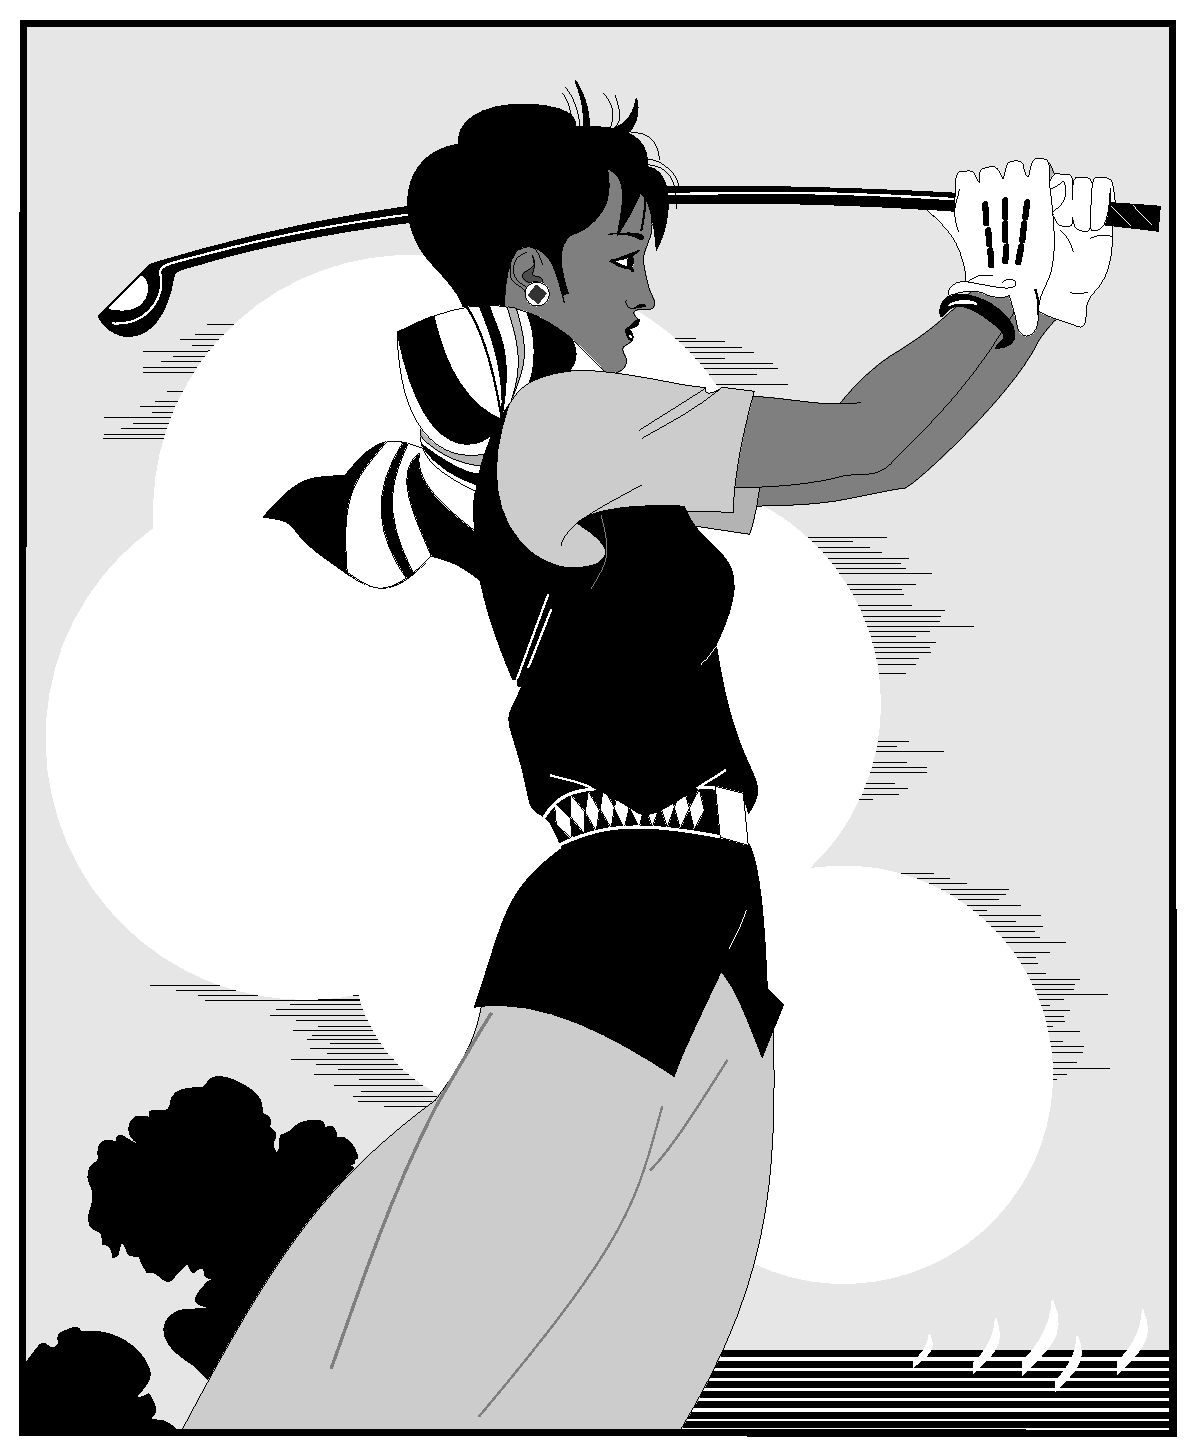
\includegraphics[width=0.2\textwidth]{golfer}}
			\fbox{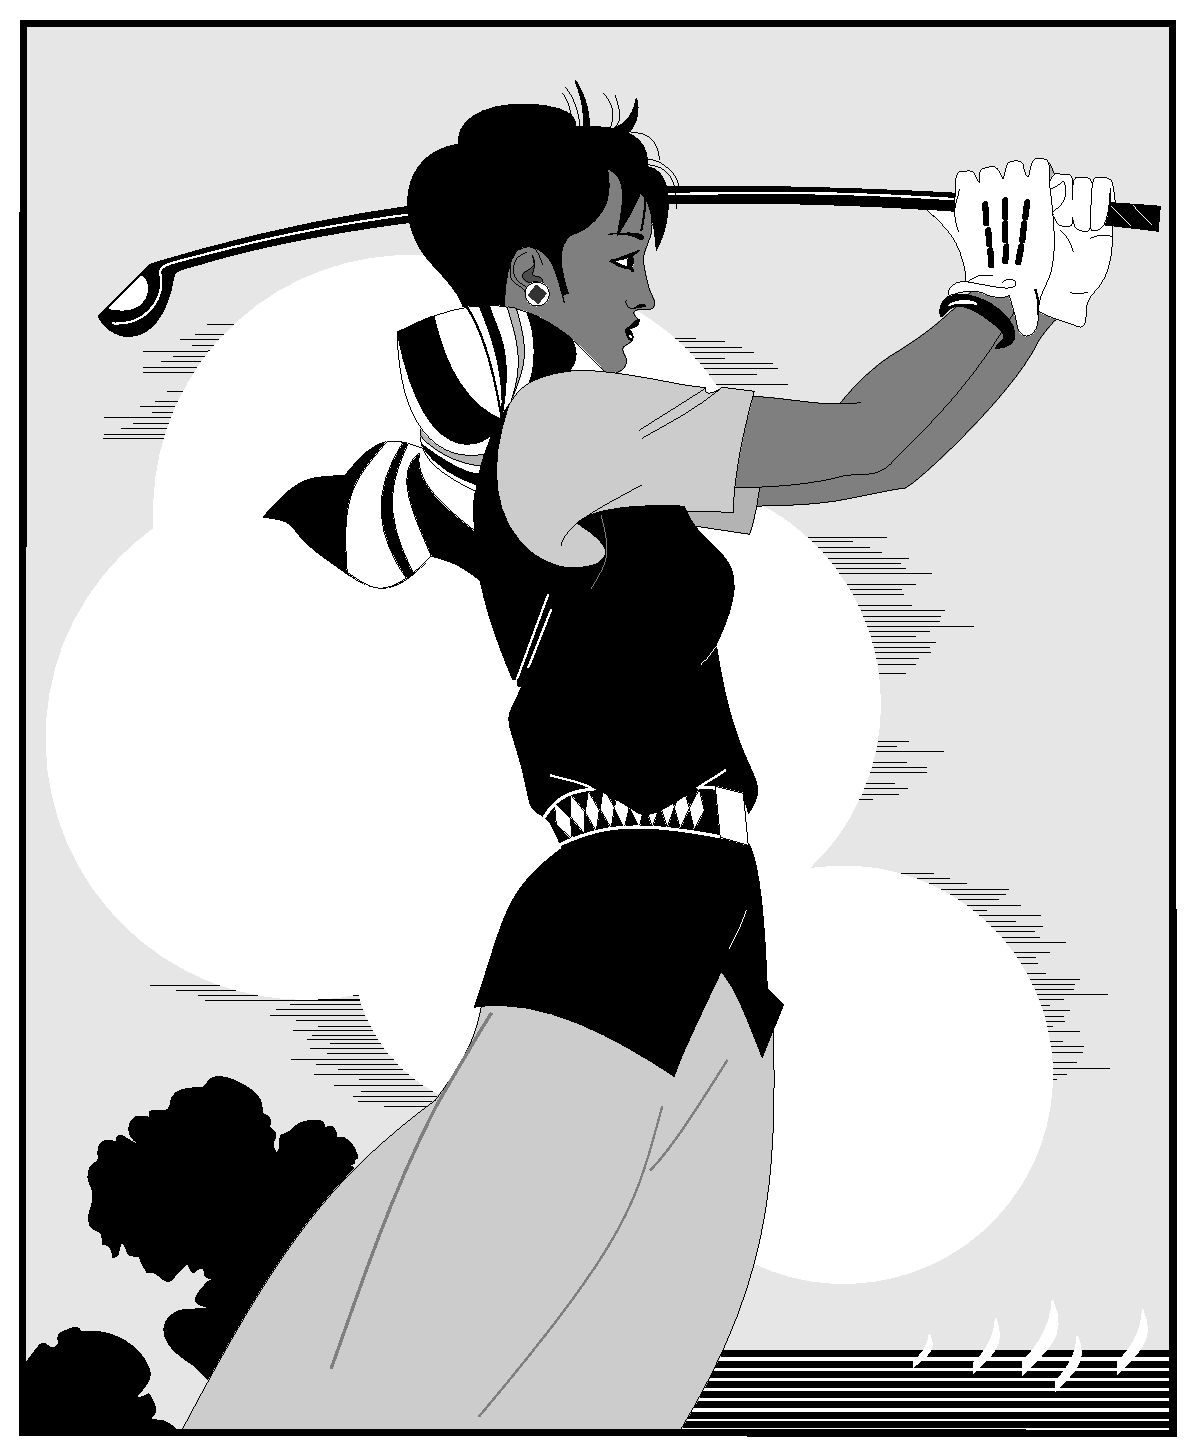
\includegraphics[width=0.2\textwidth]{golfer}}
			\fbox{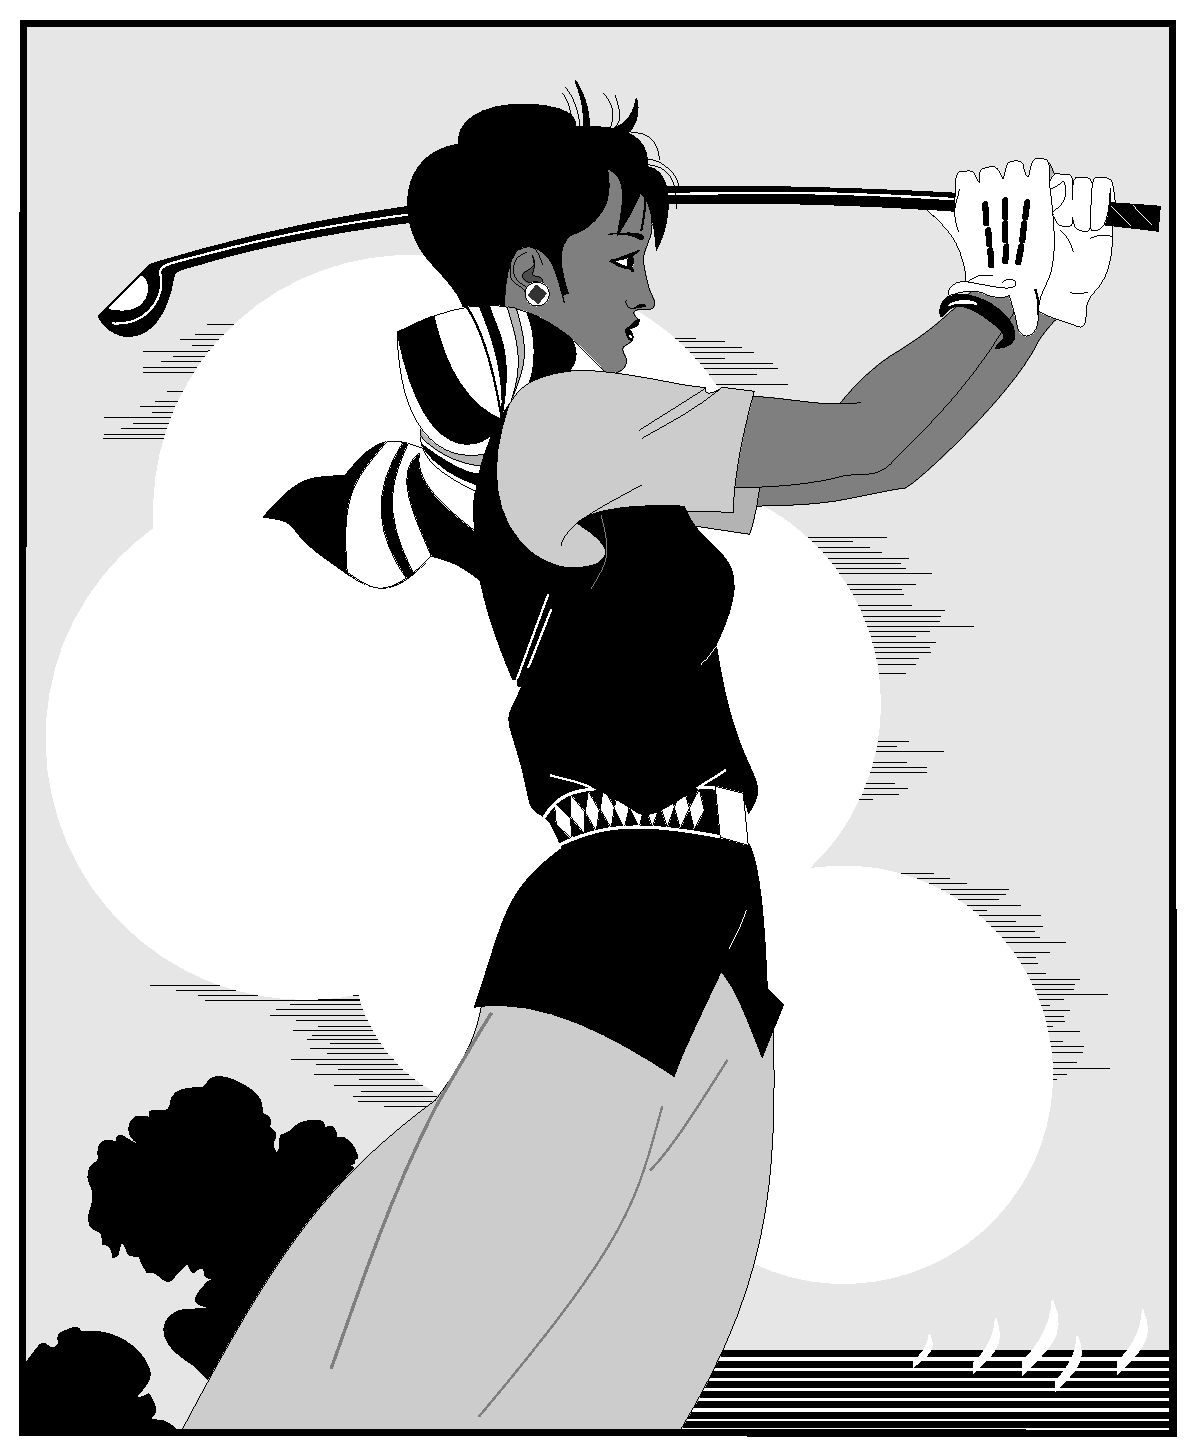
\includegraphics[width=0.2\textwidth]{golfer}}
			\fbox{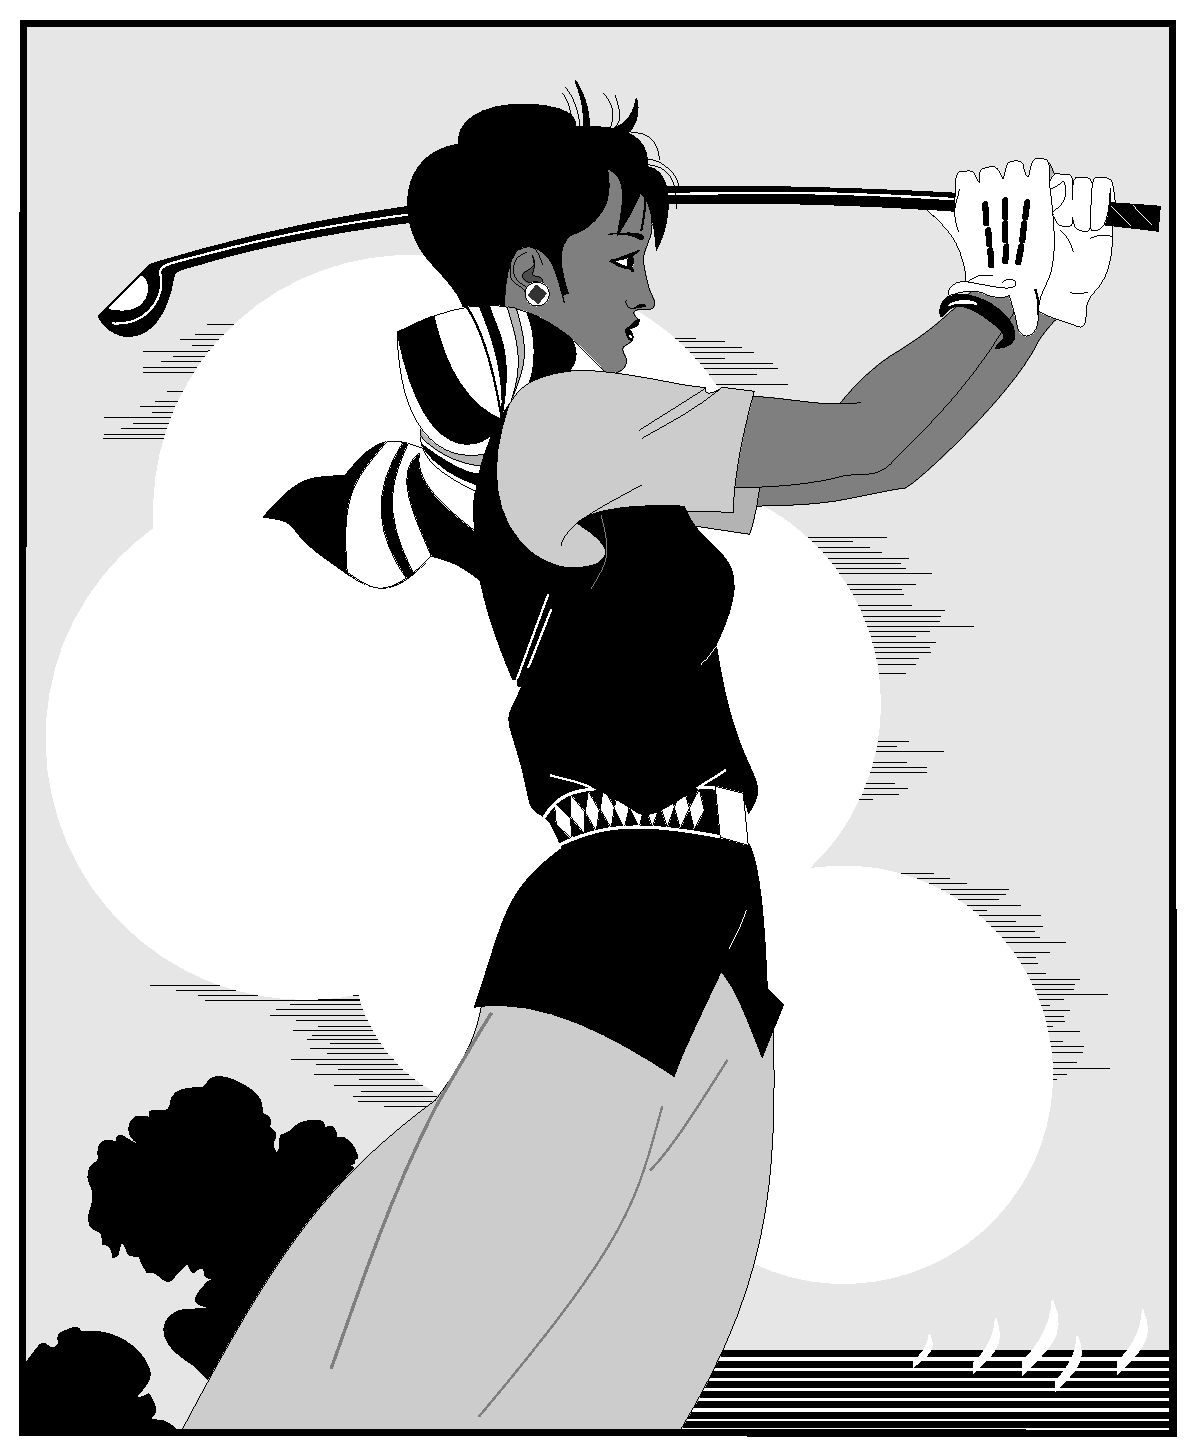
\includegraphics[width=0.2\textwidth]{golfer}}
\bicaption[golfer7]{}{打高尔夫球的人(非规范要求)}{Fig.$\!$}{The person playing golf (Not stated in the regulation)}
		\end{minipage}
	\end{sideways}
\end{figure}

\clearpage

如果不想让图片浮动到下一章节,那么在此处使用\cs{clearpage}命令。

\section{如何做出符合规范的漂亮的图}

关于作图工具在后文\ref{drawtool}中给出一些作图工具的介绍,此处不多言。
此处以R语言和Tikz为例说明如何做出符合规范的图。

\subsection{Tikz作图}

使用Tikz作图核心思想是把格式、主题、样式与内容分离,定义在全局中。
注意字体设置可以有两种选择,如果字少,用五号字,字多用小五。
使用Tikz作图不会出现字体问题,字体会自动与正文一致。

\subsection{R作图}

R是一种极具有代表性的典型的作图工具,应用广泛。
与Tikz图不同,R作图分两种情况:(1)可以转换为Tikz码;(2)不可转换为Tikz码。
第一种情况图形简单,图形中不含有很多数据点,使用R语言中的Tikz包即可。
第二种情况是图形复杂,含有海量数据点,这时候不要转成Tikz矢量图,这会使得论文体积巨大。
推荐使用pdf或png非矢量图形。
使用非矢量图形时要注意选择好字号(五号或小五),和字体(宋体、新罗马)然后选择生成图形大小,注意此时在正文中使用\cs{includegraphics}命令导入时,不要像导入矢量图那样控制图形大小,使用图形的原本的
宽度和高度,这样就确保了非矢量图形中的文字与正文一致了。

为了控制\hitszthesis\ 的大小,此处不给出具体举例。

\subsection{专业绘图工具}[Processional drawing tool]
\label{drawtool}

推荐使用tikz包,使用tikz源码绘图的好处是,图片中的字体与正文中的字体一致。具体如
何使用tikz绘图不属于模板范畴。

tikz适合用来画不需要大量实验数据支撑示意图。但R语言等专业绘图工具具有画出各种、
专业、复杂的数据图。R语言中有tikz包,能自动生成tikz码,这样tikz几乎无所不能。
对于排版有极致追求的小伙伴,可以参考
\href{http://www.texample.net/tikz/resources/}{http://www.texample.net/tikz/resources/}
中所列工具,几乎所有作图软件所作的图形都可转成tikz,然后可以自由的在tikz中修改
图中内容,定义字体等等。实现前文窝工规范中要求的图中字体的一致性的终极目标。

\lipsum[1]

\section{本章小结}[Brief summary]

\lipsum[1]


% 第3章
% !TEX root = ../main.tex

% 中英标题:\chapter{中文标题}[英文标题]
\chapter{虚拟机管理系统软件的适配}[Typesetting equations]

\section{引言}[Introduction]

\lipsum[1]

\section{对物理量符号进行注释的情况}[The condition when physical symbols
need to be annotated]

为使得对公式中物理量符号注释的转行与破折号“———”后第一个字对齐,此处最好采用表格
环境。此表格无任何线条,左对齐,且在破折号处对齐,一共有“式中”二字、物理量符号和
注释三列,表格的总宽度可选为文本宽度,因此应该采用\verb|tabularx|环境。由
\verb|tabularx|环境生成的对公式中物理量符号进行注释的公式如式(\ref{eq:1})所示。
\begin{equation}\label{eq:1}
\ddot{\bm{\rho}}-\frac{\mu}{R_{t}^{3}}\left(3\bm{R_{t}}\frac{\bm{R_{t}\rho}}{R_{t}^{2}}-\bm{\rho}\right)=\bm{a}
\end{equation}
\begin{tabularx}{\textwidth}{@{}l@{\quad}r@{———}X@{}}
式中& $\bm{\rho}$ &追踪飞行器与目标飞行器之间的相对位置矢量;\\
&  $\bm{\ddot{\rho}}$&追踪飞行器与目标飞行器之间的相对加速度;\\
&  $\bm{a}$   &推力所产生的加速度;\\
&  $\bm{R_t}$ & 目标飞行器在惯性坐标系中的位置矢量;\\
&  $\omega_{t}$ & 目标飞行器的轨道角速度;\\
\end{tabularx}\vspace{3.15bp}
由此方法生成的注释内容应紧邻待注释公式并置于其下方,因此不能将代码放入
\verb|table|浮动环境中。但此方法不能实现自动转页接排,可能会在当前页剩余空间不够
时,全部移动到下一页而导致当前页出现很大空白。因此在需要转页处理时,还请您手动将
需要转页的代码放入一个新的\verb|tabularx|环境中,将原来的一个\verb|tabularx|环境
拆分为两个\verb|tabularx|环境。

\section{子公式}[Sub-Equations]

子公式编号示例:如果需要对公式的子公式进行编号,则使用\lstinline{subeqnarray}环境:
\begin{subeqnarray}
  \label{eqw}
  \slabel{eq0}
  x & = & a \times b \\
  \slabel{eq1}
  & = & z + t\\
  \slabel{eq2}
  & = & z + t
\end{subeqnarray}

\equref{eqw}中,\lstinline{label}为整个公式的标签,\lstinline{slabel}为子公式的标签。

\section{本章小结}[Brief summary]

\lipsum[1]


% 第4章
% !TEX root = ../main.tex

% 中英标题:\chapter{中文标题}[英文标题]
\chapter{虚拟化扩展的性能评测}[Typesetting tables]

\section{引言}[Introduction]

表应有自明性。表格不加左、右边线。表的编排建议采用国际通行的三线表。表中文字用宋
体~5~号字。每个表格均应有表题(由表序和表名组成)。表序一般按章编排,如第~1~章第
一个插表的序号为“表~1-1”等。表序与表名之间空一格,表名中不允许使用标点符号,表名
后不加标点。表题置于表上,硕士学位论文只用中文,博士学位论文用中、英文两种文字居
中排写,中文在上,要求中文用宋体~5~号字,英文用新罗马字体~5~号字。表头设计应简单
明了,尽量不用斜线。表头中可采用化学符号或物理量符号。

\section{普通表格的绘制方法}[Methods of drawing normal tables]

表格应具有三线表格式,因此需要调用~booktabs~宏包,其标准格式如表~\ref{table1}~所示。
\begin{table}[htbp]
\bicaption[table1]{}{符合研究生院绘图规范的表格}{Table$\!$}{Table in agreement of the standard from graduate school}
\vspace{0.5em}\centering\wuhao
\begin{tabular}{ccccc}
\toprule[1.5pt]
$D$(in) & $P_u$(lbs) & $u_u$(in) & $\beta$ & $G_f$(psi.in)\\
\midrule[1pt]
 5 & 269.8 & 0.000674 & 1.79 & 0.04089\\
10 & 421.0 & 0.001035 & 3.59 & 0.04089\\
20 & 640.2 & 0.001565 & 7.18 & 0.04089\\
\bottomrule[1.5pt]
\end{tabular}
\end{table}
全表如用同一单位,则将单位符号移至表头右上角,加圆括号。表中数据应准确无误,书写
清楚。数字空缺的格内加横线“-”(占~2~个数字宽度)。表内文字或数字上、下或左、右
相同时,采用通栏处理方式,不允许用“〃”、“同上”之类的写法。表内文字说明,起行空一
格、转行顶格、句末不加标点。如某个表需要转页接排,在随后的各页上应重复表的编号。
编号后加“(续表)”,表题可省略。续表应重复表头。

\section{长表格的绘制方法}[Methods of drawing long tables]

长表格是当表格在当前页排不下而需要转页接排的情况下所采用的一种表格环境。若长表格
仍按照普通表格的绘制方法来获得,其所使用的\verb|table|浮动环境无法实现表格的换页
接排功能,表格下方过长部分会排在表格第1页的页脚以下。为了能够实现长表格的转页接
排功能,需要调用~longtable~宏包,由于长表格是跨页的文本内容,因此只需要单独的
\verb|longtable|环境,所绘制的长表格的格式如表~\ref{table2}~所示。

注意,长表格双语标题的格式。

\vspace{-1.5bp}
\ltfontsize{\wuhao[1.667]}
\wuhao[1.667]\begin{longtable}{ccc}%
\longbionenumcaption{}{{\wuhao 中国省级行政单位一览
}\label{table2}}{Table$\!$}{}{{\wuhao Overview of the provincial administrative
unit of China}}{-0.5em}{3.15bp}\\
%\caption{\wuhao 中国省级行政单位一览}\\
\toprule[1.5pt] 名称 & 简称 & 省会或首府  \\ \midrule[1pt]
\endfirsthead
\multicolumn{3}{r}{表~\thetable(续表)}\vspace{0.5em}\\
\toprule[1.5pt] 名称 & 简称 & 省会或首府  \\ \midrule[1pt]
\endhead
\bottomrule[1.5pt]
\endfoot
北京市 & 京 & 北京\\
天津市 & 津 & 天津\\
河北省 & 冀 & 石家庄市\\
山西省 & 晋 & 太原市\\
内蒙古自治区 & 蒙 & 呼和浩特市\\
辽宁省 & 辽 & 沈阳市\\
吉林省 & 吉 & 长春市\\
黑龙江省 & 黑 & 哈尔滨市\\
上海市 & 沪/申 & 上海\\
江苏省 & 苏 & 南京市\\
浙江省 & 浙 & 杭州市\\
安徽省 & 皖 & 合肥市\\
福建省 & 闽 & 福州市\\
江西省 & 赣 & 南昌市\\
山东省 & 鲁 & 济南市\\
河南省 & 豫 & 郑州市\\
湖北省 & 鄂 & 武汉市\\
湖南省 & 湘 & 长沙市\\
广东省 & 粤 & 广州市\\
广西壮族自治区 & 桂 & 南宁市\\
海南省 & 琼 & 海口市\\
重庆市 & 渝 & 重庆\\
四川省 & 川/蜀 & 成都市\\
贵州省 & 黔/贵 & 贵阳市\\
云南省 & 云/滇 & 昆明市\\
西藏自治区 & 藏 & 拉萨市\\
陕西省 & 陕/秦 & 西安市\\
甘肃省 & 甘/陇 & 兰州市\\
青海省 & 青 & 西宁市\\
宁夏回族自治区 & 宁 & 银川市\\
新疆维吾尔自治区 & 新 & 乌鲁木齐市\\
香港特别行政区 & 港 & 香港\\
澳门特别行政区 & 澳 & 澳门\\
台湾省 & 台 & 台北市\\
\end{longtable}\normalsize
\vspace{-1em}

此长表格~\ref{table2}~第~2~页的标题“编号(续表)”和表头是通过代码自动添加上去的,无需人工添加,若表格在页面中的竖直位置发生了变化,长表格在第~2~页
及之后各页的标题和表头位置能够始终处于各页的最顶部,也无需人工调整,\LaTeX~系统的这一优点是~word~等软件所无法比拟的。

\section{列宽可调表格的绘制方法}[Methods of drawing tables with adjustable-width columns]
论文中能用到列宽可调表格的情况共有两种,一种是当插入的表格某一单元格内容过长以至
于一行放不下的情况,另一种是当对公式中首次出现的物理量符号进行注释的情况,这两种
情况都需要调用~tabularx~宏包。下面将分别对这两种情况下可调表格的绘制方法进行阐述
。
\subsection{表格内某单元格内容过长的情况}[The condition when the contents in
some cells of tables are too long]
首先给出这种情况下的一个例子如表~\ref{table3}~所示。
\begin{table}[htbp]
  \centering
\bicaption[table3]{}{最小的三个正整数的英文表示法}{Table$\!$}{The English construction of the smallest three positive integral numbers}\vspace{0.5em}\wuhao
\begin{tabularx}{0.7\textwidth}{llX}
\toprule[1.5pt]
Value & Name & Alternate names, and names for sets of the given size\\\midrule[1pt]
1 & One & ace, single, singleton, unary, unit, unity\\
2 & Two & binary, brace, couple, couplet, distich, deuce, double, doubleton, duad, duality, duet, duo, dyad, pair, snake eyes, span, twain, twosome, yoke\\
3 & Three & deuce-ace, leash, set, tercet, ternary, ternion, terzetto, threesome, tierce, trey, triad, trine, trinity, trio, triplet, troika, hat-trick\\\bottomrule[1.5pt]
\end{tabularx}
\end{table}
tabularx环境共有两个必选参数:第1个参数用来确定表格的总宽度,第2个参数用来确定每
列格式,其中标为X的项表示该列的宽度可调,其宽度值由表格总宽度确定。标为X的列一般
选为单元格内容过长而无法置于一行的列,这样使得该列内容能够根据表格总宽度自动分行
。若列格式中存在不止一个X项,则这些标为X的列的列宽相同,因此,一般不将内容较短的
列设为X。标为X的列均为左对齐,因此其余列一般选为l(左对齐),这样可使得表格美观
,但也可以选为c或r。

\subsection{排版横版表格的举例}[An example of landscape table]

横版表格如\tabref{table4}所示。

\begin{table}[p]
\centering
  \begin{sideways}
    \begin{minipage}{\textheight}
      \bicaption[table4]{}{不在规范中规定的横版表格}{Table$\!$}{A table style which is not stated in the regulation}
      \vspace{0.5em}\centering\wuhao
      \begin{tabular}{ccccc}
        \toprule[1.5pt]
        $D$(in) & $P_u$(lbs) & $u_u$(in) & $\beta$ & $G_f$(psi.in)\\
        \midrule[1pt]
        5 & 269.8 & 0.000674 & 1.79 & 0.04089\\
        10 & 421.0 & 0.001035 & 3.59 & 0.04089\\
        20 & 640.2 & 0.001565 & 7.18 & 0.04089\\
        \bottomrule[1.5pt]
      \end{tabular}
    \end{minipage}
  \end{sideways}
\end{table}

\section{本章小结}[Brief summary]

\lipsum[1]


% 第5章
% !TEX root = ../main.tex

\chapter{引用参考文献}[Cite reference]

\section{引言}[Introduction]

\lipsum[1]

\section{参考文献引用方法}[How to cite the reference]

\sindex[china]{du!段誉}引文标注遵照GB/T7714-2005,采用顺序编码制。正文中引用文献的标示应置于所引内容最后一个字的右上角,所引文献编号用阿拉伯数字置于方括号“[ ]”中,用小4号字体的上角标。要求:

(1)引用单篇文献时,如“二次铣削\cite{ren2010}”。

(2)同一处引用多篇文献时,各篇文献的序号在方括号内全部列出,各序号间用“,”,如
遇连续序号,可标注讫序号。如,…形成了多种数学模型\cite{Gravagne2003,ren2010}…
注意此处添加\cs{inlinecite}中文空格\inlinecite{Gravagne2003,ren2010},可以在cfg文件中修改空格类型。

(3)多次引用同一文献时,在文献序号的“[ ]”后标注引文页码。如,…间质细胞CAMP含量
测定\cite[100-197]{Gravagne2003}…。…含量测定方法规定
\cite[92]{Gravagne2003}…。

(4)当提及的参考文献为文中直接说明时,则用小4号字与正文排齐,如“由文献\inlinecite{webster2010}可知”

(5)多\cite{liu2016}引\cite{fu2018}用\cite{zhai2015}一\cite{yao2015}些\cite{jones2006}参\cite{mcmahan2005}考\cite{jones2004}文献以生成附录参考文献。

\section{本章小结}[Brief summary]

\lipsum[1]


% 第6章
% !TEX root = ../main.tex

% 中英标题:\chapter{中文标题}[英文标题]
\chapter{补充说明}[Complements]

\section{引言}[Introduction]

这是 \hitszthesis\ 的示例文档,基本上覆盖了模板中所有格式的设置。建议大家在使用模
板之前,除了阅读《\hitszthesis\:哈尔滨工业大学学位论文模板》\footnote{即
hitszthesis.pdf文件},本示例文档也最好能看一看。此示例文档尽量使用到所有的排版格式
,然而对于一些不在我工规范中规定的文档,理论上是由用户自由发挥,这里不给出样例
。需要另行载入的宏包和自定义命令在文件`hitszthesis.sty'中有示例,这里不列举。

\section{关于数字}[Number]

按《关于出版物上数字用法的试行规定》(1987年1月1日国家语言文字工作委员会等7个单位公布),除习惯用中文数字表示的以外,一般数字均用阿拉伯数字。
(1)公历的世纪、年代、年、月、日和时刻一律用阿拉伯数字,如20世纪,80年代,4时3刻等。年号要用四位数,如1989年,不能用89年。
(2)记数与计算(含正负整数、分数、小数、百分比、约数等)一律用阿拉伯数字,如3/4,4.5\%,10个月,500多种等。
(3)一个数值的书写形式要照顾到上下文。不是出现在一组表示科学计量和具有统计意义数字中的一位数可以用汉字,如一个人,六条意见。星期几一律用汉字,如星期六。邻近两个数字并列连用,表示概数,应该用汉字数字,数字间不用顿号隔开,如三五天,七八十种,四十五六岁,一千七八百元等。
(4)数字作为词素构成定型的词、词组、惯用语、缩略语等应当使用汉字。如二倍体,三叶虫,第三世界,“七五”规划,相差十万八千里等。
(5)5位以上的数字,尾数零多的,可改写为以万、亿为单位的数。一般情况下不得以十、百、千、十万、百万、千万、十亿、百亿、千亿作为单位。如~\num{345000000}~公里可改写为3.45亿公里或~\num{34500}~万公里,但不能写为3亿~\num{4500}~万公里或3亿4千5百万公里。
(6)数字的书写不必每格一个数码,一般每两数码占一格,数字间分节不用分位号“,”,凡4位或4位以上的数都从个位起每3位数空半个数码(1/4汉字)。“\num{3000000}”,不要写成“3,000,000”,小数点后的数从小数点起向右按每三位一组分节。一个用阿拉伯数字书写的多位数不能从数字中间转行。
(7)数量的增加或减少要注意下列用词的概念:1)增加为(或增加到)过去的二倍,即过去为一,现在为二;2)增加(或增加了)二倍,即过去为一,现在为三;3)超额80\%,即定额为100,现在为180;4)降低到80\%,即过去为100,现在为80;5)降低(或降低了)80\%,即原来为100,现在为20;6)为原数的1/4,即原数为4,现在为1,或原数为1,现在为0.25。
应特别注意在表达数字减小时,不宜用倍数,而应采用分数。如减少为原来的1/2,1/3等。

\section{索引示例}[Index]

为便于检索文中内容,可编制索引置于论文之后(根据需要决定是否设置)。索引以论文中
的专业词语为检索线索,指出其相关内容的所在页码。索引用中、英两种文字书写,中文在
前。\sindex[china]{qi!乔峰}\sindex[english]{Xu Zhu}\sindex[english]{Qiao Feng}
中文按各词汉语拼音第一个字母排序,英文按该词第一个英文字母排序。

\section{术语排版举例}[Glossaries and index]

术语的定义和使用可以结合索引,灵活使用。例如,\gtssbp 是一种应用于狄利克雷过程抽样的算法。下次出现将是另一种格式:\gtssbp 。还可以切换单复数例如:\gscna ,下次出现为:\gscnas 。此处体现了\LaTeX\ 格式内容分离的优势。

\section{定理和定义等}[Theorem]

\begin{theorem}[\cite{ren2010}]
宇宙大爆炸是一种爆炸。
\end{theorem}
\begin{definition}[(霍金)]
宇宙大爆炸是一种爆炸。
\end{definition}
\begin{assumption}
宇宙大爆炸是一种爆炸。
\end{assumption}
\begin{lemma}
宇宙大爆炸是一种爆炸。
\end{lemma}
\begin{corollary}
宇宙大爆炸是一种爆炸。
\end{corollary}
\begin{exercise}
宇宙大爆炸是一种爆炸。
\end{exercise}
\begin{problem}[(Albert Einstein)]
宇宙大爆炸是一种爆炸。
\end{problem}
\begin{remark}
宇宙大爆炸是一种爆炸。
\end{remark}
\begin{axiom}[(爱因斯坦)]
宇宙大爆炸是一种爆炸。
\end{axiom}
\begin{conjecture}
宇宙大爆炸是一种爆炸。
\end{conjecture}

\lipsum[1]

\section{其他杂项}[Miscellaneous]

\subsection{右翻页}[Open right]

对于双面打印的论文,强制使每章的标题页出现右手边为右翻页。规范中没有明确规定是否是右翻页打印。模板给出了右翻页选项。为了应对用户的个人喜好,在希望设置成右翻页的位置之前添加\cs{cleardoublepage}命令即可。

\subsection{算法}[Algorithms]

算法不在规范中要求,在hitszthesis.sty中有相关定义,一个例子如算法\ref{alg:rerank}所示。
\begin{algorithm}
  \DontPrintSemicolon
  \wuhao
  \caption{混合重排算法}
  \label{alg:rerank}
  \KwData{$A$:待重排的元素集合 \newline
  $\alpha$: 对多样性,相关性作折中的权重因子}
  \KwResult{$A_k$: a subset of $A$ of size k}
\end{algorithm}

\subsection{脚注}[Footnotes]

不在再规范\footnote{规范是指\PGR\ 和\UGR}中要求,模板默认使用清华大学的格式。

\subsection{源码}[Source code]

也不在再规范中要求。如果有需要最好使用minted包,但在编译的时候需要添加“-shell-escape”选项且安装pygmentize软件,这些不在模板中默认载入,如果需要自行载入。

\subsection{思源宋体}[Siyuan font]
如果要使用思源字体,需要思源字体的定义文件,此文件请到模板的开发版网址github:
\href{https://gihitb.com/YangLaTeX/hitszthesis}{https://gihitb.com/YangLaTeX/hitszthesis}
处下载。

\subsection{术语词汇管理}[Manage glossaries]

推荐使用glossaries包管理术语、缩略语,可以自动生成首次全写,非首次缩写。

\section{本章小结}[Brief summary]

\lipsum[2]


% 开始写正文之后的部分
\backmatter

%%%% \begin{本科书序} %%%% 这是一个假的环境,本科请用这里的内容

% 结论
% !Mode:: "TeX:UTF-8" 
\begin{conclusions}

本文围绕着为RISC-V开源处理器"香山"的南湖架构添加虚拟化扩展,
讲述了对虚拟化微架构、系统软件和调试工具三个方面的研究。
第一,在虚拟化微架构上,扩展了“香山”特权控制和虚拟内存两部分的设计,从而实现了虚拟化扩展。
特别是虚拟内部分,通过添加第二阶段地址翻译单元、复用二级页表缓存等能够加快页表翻译的微架构。
第二,在添加虚拟化扩展的“香山”上尝试启动Linux和虚拟机管理系统KVM。
在FPGA加速仿真工具REMU的调试帮助下,Linux能够顺利启动。
但是在启动KVM虚拟机时,由于硬件设计还是存在尚未发掘的错误而失败。
第三,为了找出错误,尝试了基于纯软件逻辑仿真的差分测试以及基于FPGA的仿真加速平台等调试工具。
但由于软硬件联合调试的复杂性以及现有调试工具的能力限制,问题未能解决。
因此,对扩展现有调试工具的能力方面进行了探索:
基于纯软件仿真的差分测试工具,可以联合使用体系结构信息检查点,跳过不必要的操作系统仿真步骤。
基于FPGA的仿真加速工具,可以在差分测试框架中重放微架构检查点,或者是将差分测试硬件化在FPGA中。

\end{conclusions}


% 参考文献
\bibliographystyle{hitszthesis}
\bibliography{reference}

% 发表文章
% !Mode:: "TeX:UTF-8" 
\begin{publication}
\noindent\textbf{发表的相关论文}
\begin{publist}
\item	XXX,XXX. Static Oxidation Model of Al-Mg/C Dissipation Thermal Protection Materials[J]. Rare Metal Materials and Engineering, 2010, 39(Suppl. 1): 520-524.(SCI~收录,IDS号为~669JS,IF=0.16)
\item XXX,XXX. 精密超声振动切削单晶铜的计算机仿真研究[J]. 系统仿真学报,2007,19(4):738-741,753.(EI~收录号:20071310514841)
\item XXX,XXX. 局部多孔质气体静压轴向轴承静态特性的数值求解[J]. 摩擦学学报,2007(1):68-72.(EI~收录号:20071510544816)
\item XXX,XXX. 硬脆光学晶体材料超精密切削理论研究综述[J]. 机械工程学报,2003,39(8):15-22.(EI~收录号:2004088028875)
\item XXX,XXX. 基于遗传算法的超精密切削加工表面粗糙度预测模型的参数辨识以及切削参数优化[J]. 机械工程学报,2005,41(11):158-162.(EI~收录号:2006039650087)
\item XXX,XXX. Discrete Sliding Mode Cintrok with Fuzzy Adaptive Reaching Law on 6-PEES Parallel Robot[C]. Intelligent System Design and Applications, Jinan, 2006: 649-652.(EI~收录号:20073210746529)
\end{publist}

\noindent\textbf{(二)申请及已获得的专利(无专利时此项不必列出)}
\begin{publist}
\item XXX,XXX. 一种温热外敷药制备方案:中国,88105607.3[P]. 1989-07-26.
\end{publist}

\noindent\textbf{(三)参与的科研项目及获奖情况}
\begin{publist}
\item	XXX,XXX. XX~气体静压轴承技术研究, XX~省自然科学基金项目.课题编号:XXXX.
\item XXX,XXX. XX~静载下预应力混凝土房屋结构设计统一理论. 黑江省科学技术二等奖, 2007.
\end{publist}
%\vfill
%\hangafter=1\hangindent=2em\noindent
%\setlength{\parindent}{2em}
\end{publication}


% 授权
\authorization

% 授权页为扫描的PDF文件(scan.pdf),与上面的命令互斥
% \authorization[scan.pdf]

% 致谢
% !TEX root = ../main.tex

% 致谢
\begin{acknowledgements}
衷心感谢导师~XXX~教授对本人的精心指导。他的言传身教将使我终生受益。

……

感谢哈深\LaTeX{}论文模板\hitszthesis\ !

\end{acknowledgements}


% 附录
% 设置附录部分只包含页眉
% \SetAppendixWithOnlyHeadings
% 设置附录部分页码从1开始编号的命令在<back/appendix01.tex>里
\begin{appendix}
  % !TEX root = ../main.tex

% 附录1
\chapter{外文资料翻译}
% 设置附录页码从1开始编号
% \SetPageNumberingFromOne

\title{英文资料的中文标题}

{\heiti 摘要:} 本章为外文资料翻译内容。如果有摘要可以直接写上来,这部分好像没有
明确的规定。

\section{单目标规划}
北冥有鱼,其名为鲲。鲲之大,不知其几千里也。化而为鸟,其名为鹏。鹏之背,不知其几
千里也。怒而飞,其翼若垂天之云。是鸟也,海运则将徙于南冥。南冥者,天池也。
\begin{equation}\tag*{(123)}
 p(y|\mathbf{x}) = \frac{p(\mathbf{x},y)}{p(\mathbf{x})}=
\frac{p(\mathbf{x}|y)p(y)}{p(\mathbf{x})}
\end{equation}

吾生也有涯,而知也无涯。以有涯随无涯,殆已!已而为知者,殆而已矣!为善无近名,为
恶无近刑,缘督以为经,可以保身,可以全生,可以养亲,可以尽年。

\subsection{线性规划}
庖丁为文惠君解牛,手之所触,肩之所倚,足之所履,膝之所倚,砉然响然,奏刀騞然,莫
不中音,合于桑林之舞,乃中经首之会。
\begin{table}[ht]
  \centering
  \wuhao
  \caption*{表~1\hskip1em 这是手动编号但不出现在索引中的一个表格例子}
  \label{tab:badtabular3}
  \begin{tabular}[c]{|m{1.5cm}|c|c|c|c|c|c|}\hline
    \multicolumn{2}{|c|}{Network Topology} & \# of nodes &
    \multicolumn{3}{c|}{\# of clients} & Server \\\hline
    GT-ITM & Waxman Transit-Stub & 600 &
    \multirow{2}{2em}{2\%}&
    \multirow{2}{2em}{10\%}&
    \multirow{2}{2em}{50\%}&
    \multirow{2}{1.2in}{Max. Connectivity}\\\cline{1-3}
    \multicolumn{2}{|c|}{Inet-2.1} & 6000 & & & &\\\hline
    & \multicolumn{2}{c|}{ABCDEF} &\multicolumn{4}{c|}{} \\\hline
\end{tabular}
\end{table}

文惠君曰:“嘻,善哉!技盖至此乎?”庖丁释刀对曰:“臣之所好者道也,进乎技矣。始臣之
解牛之时,所见无非全牛者;三年之后,未尝见全牛也;方今之时,臣以神遇而不以目视,
官知止而神欲行。依乎天理,批大郤,导大窾,因其固然。技经肯綮之未尝,而况大坬乎!
良庖岁更刀,割也;族庖月更刀,折也;今臣之刀十九年矣,所解数千牛矣,而刀刃若新发
于硎。彼节者有间而刀刃者无厚,以无厚入有间,恢恢乎其于游刃必有余地矣。是以十九年
而刀刃若新发于硎。虽然,每至于族,吾见其难为,怵然为戒,视为止,行为迟,动刀甚微,
謋然已解,如土委地。提刀而立,为之而四顾,为之踌躇满志,善刀而藏之。”

文惠君曰:“善哉!吾闻庖丁之言,得养生焉。”


\subsection{非线性规划}
孔子与柳下季为友,柳下季之弟名曰盗跖。盗跖从卒九千人,横行天下,侵暴诸侯。穴室枢
户,驱人牛马,取人妇女。贪得忘亲,不顾父母兄弟,不祭先祖。所过之邑,大国守城,小
国入保,万民苦之。孔子谓柳下季曰:“夫为人父者,必能诏其子;为人兄者,必能教其弟。
若父不能诏其子,兄不能教其弟,则无贵父子兄弟之亲矣。今先生,世之才士也,弟为盗
跖,为天下害,而弗能教也,丘窃为先生羞之。丘请为先生往说之。”

柳下季曰:“先生言为人父者必能诏其子,为人兄者必能教其弟,若子不听父之诏,弟不受
兄之教,虽今先生之辩,将奈之何哉?且跖之为人也,心如涌泉,意如飘风,强足以距敌,
辩足以饰非。顺其心则喜,逆其心则怒,易辱人以言。先生必无往。”

孔子不听,颜回为驭,子贡为右,往见盗跖。

\subsection{整数规划}
盗跖乃方休卒徒大山之阳,脍人肝而餔之。孔子下车而前,见谒者曰:“鲁人孔丘,闻将军
高义,敬再拜谒者。”谒者入通。盗跖闻之大怒,目如明星,发上指冠,曰:“此夫鲁国之
巧伪人孔丘非邪?为我告之:尔作言造语,妄称文、武,冠枝木之冠,带死牛之胁,多辞缪
说,不耕而食,不织而衣,摇唇鼓舌,擅生是非,以迷天下之主,使天下学士不反其本,妄
作孝弟,而侥幸于封侯富贵者也。子之罪大极重,疾走归!不然,我将以子肝益昼餔之膳。”
  % !TEX root = ../main.tex

% 附录2
\chapter{外文资料原文}
\label{cha:engorg}

\title{The title of the English paper}

\textbf{Abstract:} As one of the most widely used techniques in operations
research, \emph{ mathematical programming} is defined as a means of maximizing a
quantity known as \emph{bjective function}, subject to a set of constraints
represented by equations and inequalities. Some known subtopics of mathematical
programming are linear programming, nonlinear programming, multiobjective
programming, goal programming, dynamic programming, and multilevel
programming$^{[1]}$.

It is impossible to cover in a single chapter every concept of mathematical
programming. This chapter introduces only the basic concepts and techniques of
mathematical programming such that readers gain an understanding of them
throughout the book$^{[2,3]}$.


\section{Single-Objective Programming}
The general form of single-objective programming (SOP) is written
as follows,
\begin{equation}\tag*{(123)} % 如果附录中的公式不想让它出现在公式索引中,那就请
                             % 用 \tag*{xxxx}
\left\{\begin{array}{l}
\max \,\,f(x)\\[0.1 cm]
\mbox{subject to:} \\ [0.1 cm]
\qquad g_j(x)\le 0,\quad j=1,2,\cdots,p
\end{array}\right.
\end{equation}
which maximizes a real-valued function $f$ of
$x=(x_1,x_2,\cdots,x_n)$ subject to a set of constraints.

\newtheorem{mpdef}{Definition}[chapter]
\begin{mpdef}
In SOP, we call $x$ a decision vector, and
$x_1,x_2,\cdots,x_n$ decision variables. The function
$f$ is called the objective function. The set
\begin{equation}\tag*{(456)} % 这里同理,其它不再一一指定。
S=\left\{x\in\Re^n\bigm|g_j(x)\le 0,\,j=1,2,\cdots,p\right\}
\end{equation}
is called the feasible set. An element $x$ in $S$ is called a
feasible solution.
\end{mpdef}

\newtheorem{mpdefop}[mpdef]{Definition}
\begin{mpdefop}
A feasible solution $x^*$ is called the optimal
solution of SOP if and only if
\begin{equation}
f(x^*)\ge f(x)
\end{equation}
for any feasible solution $x$.
\end{mpdefop}

One of the outstanding contributions to mathematical programming was known as
the Kuhn-Tucker conditions\ref{eq:ktc}. In order to introduce them, let us give
some definitions. An inequality constraint $g_j(x)\le 0$ is said to be active at
a point $x^*$ if $g_j(x^*)=0$. A point $x^*$ satisfying $g_j(x^*)\le 0$ is said
to be regular if the gradient vectors $\nabla g_j(x)$ of all active constraints
are linearly independent.

Let $x^*$ be a regular point of the constraints of SOP and assume that all the
functions $f(x)$ and $g_j(x),j=1,2,\cdots,p$ are differentiable. If $x^*$ is a
local optimal solution, then there exist Lagrange multipliers
$\lambda_j,j=1,2,\cdots,p$ such that the following Kuhn-Tucker conditions hold,
\begin{equation}
\label{eq:ktc}
\left\{\begin{array}{l}
    \nabla f(x^*)-\sum\limits_{j=1}^p\lambda_j\nabla g_j(x^*)=0\\[0.3cm]
    \lambda_jg_j(x^*)=0,\quad j=1,2,\cdots,p\\[0.2cm]
    \lambda_j\ge 0,\quad j=1,2,\cdots,p.
\end{array}\right.
\end{equation}
If all the functions $f(x)$ and $g_j(x),j=1,2,\cdots,p$ are convex and
differentiable, and the point $x^*$ satisfies the Kuhn-Tucker conditions
(\ref{eq:ktc}), then it has been proved that the point $x^*$ is a global optimal
solution of SOP.

\subsection{Linear Programming}
\label{sec:lp}

If the functions $f(x),g_j(x),j=1,2,\cdots,p$ are all linear, then SOP is called
a {\em linear programming}.

The feasible set of linear is always convex. A point $x$ is called an extreme
point of convex set $S$ if $x\in S$ and $x$ cannot be expressed as a convex
combination of two points in $S$. It has been shown that the optimal solution to
linear programming corresponds to an extreme point of its feasible set provided
that the feasible set $S$ is bounded. This fact is the basis of the {\em simplex
  algorithm} which was developed by Dantzig as a very efficient method for
solving linear programming.
\begin{table}[ht]
  \centering
  \appendixcaption{Table~1\hskip1em This is an example for manually numbered table, which
    would not appear in the list of tables}
  \label{tab:badtabular2}
  \wuhao
  \begin{tabular}[c]{|m{1.5cm}|c|c|c|c|c|c|}\hline
    \multicolumn{2}{|c|}{Network Topology} & \# of nodes &
    \multicolumn{3}{c|}{\# of clients} & Server \\\hline
    GT-ITM & Waxman Transit-Stub & 600 &
    \multirow{2}{2em}{2\%}&
    \multirow{2}{2em}{10\%}&
    \multirow{2}{2em}{50\%}&
    \multirow{2}{1.2in}{Max. Connectivity}\\\cline{1-3}
    \multicolumn{2}{|c|}{Inet-2.1} & 6000 & & & &\\\hline
    & \multicolumn{2}{c|}{ABCDEF} &\multicolumn{4}{c|}{} \\\hline
  \end{tabular}
\end{table}

Roughly speaking, the simplex algorithm examines only the extreme points of the
feasible set, rather than all feasible points. At first, the simplex algorithm
selects an extreme point as the initial point. The successive extreme point is
selected so as to improve the objective function value. The procedure is
repeated until no improvement in objective function value can be made. The last
extreme point is the optimal solution.

% 附录算法请用这个新环境 <algorithmen>
\begin{algorithmen}
  \wuhao
  \DontPrintSemicolon
  \KwData{$G=(X,U)$ such that $G^{tc}$ is an order.}
  \KwResult{$G’=(X,V)$ with $V\subseteq U$ such that $G’^{tc}$ is an interval order.}
  \caption{\textsc{Fast}SLAM}
\end{algorithmen}

\subsection{Nonlinear Programming}

If at least one of the functions $f(x),g_j(x),j=1,2,\cdots,p$ is nonlinear, then
SOP is called a {\em nonlinear programming}.

A large number of classical optimization methods have been developed to treat
special-structural nonlinear programming based on the mathematical theory
concerned with analyzing the structure of problems.

Now we consider a nonlinear programming which is confronted solely with
maximizing a real-valued function with domain $\Re^n$.  Whether derivatives are
available or not, the usual strategy is first to select a point in $\Re^n$ which
is thought to be the most likely place where the maximum exists. If there is no
information available on which to base such a selection, a point is chosen at
random. From this first point an attempt is made to construct a sequence of
points, each of which yields an improved objective function value over its
predecessor. The next point to be added to the sequence is chosen by analyzing
the behavior of the function at the previous points. This construction continues
until some termination criterion is met. Methods based upon this strategy are
called {\em ascent methods}, which can be classified as {\em direct methods},
{\em gradient methods}, and {\em Hessian methods} according to the information
about the behavior of objective function $f$. Direct methods require only that
the function can be evaluated at each point. Gradient methods require the
evaluation of first derivatives of $f$. Hessian methods require the evaluation
of second derivatives. In fact, there is no superior method for all
problems. The efficiency of a method is very much dependent upon the objective
function.

\subsection{Integer Programming}

{\em Integer programming} is a special mathematical programming in which all of
the variables are assumed to be only integer values. When there are not only
integer variables but also conventional continuous variables, we call it {\em
  mixed integer programming}. If all the variables are assumed either 0 or 1,
then the problem is termed a {\em zero-one programming}. Although integer
programming can be solved by an {\em exhaustive enumeration} theoretically, it
is impractical to solve realistically sized integer programming problems. The
most successful algorithm so far found to solve integer programming is called
the {\em branch-and-bound enumeration} developed by Balas (1965) and Dakin
(1965). The other technique to integer programming is the {\em cutting plane
  method} developed by Gomory (1959).

\hfill\textit{Uncertain Programming\/}\quad(\textsl{BaoDing Liu, 2006.2})

\section*{References}
\noindent{\itshape NOTE: These references are only for demonstration. They are
  not real citations in the original text.}

\begin{translationbib}
\item Donald E. Knuth. The \TeX book. Addison-Wesley, 1984. ISBN: 0-201-13448-9
\item Paul W. Abrahams, Karl Berry and Kathryn A. Hargreaves. \TeX\ for the
  Impatient. Addison-Wesley, 1990. ISBN: 0-201-51375-7
\item David Salomon. The advanced \TeX book.  New York : Springer, 1995. ISBN:0-387-94556-3
\end{translationbib}

  % !TEX root = ../main.tex

% 附录3
\chapter{其它附录}

其他的附录如数据、代码等,可以放在这里。

\end{appendix}

%%%% \end{本科书序}


%%%% \begin{硕博书序} %%%% 这是一个假的环境,硕、博请用这里的内容

% % 结论
% % !Mode:: "TeX:UTF-8" 
\begin{conclusions}

本文围绕着为RISC-V开源处理器"香山"的南湖架构添加虚拟化扩展,
讲述了对虚拟化微架构、系统软件和调试工具三个方面的研究。
第一,在虚拟化微架构上,扩展了“香山”特权控制和虚拟内存两部分的设计,从而实现了虚拟化扩展。
特别是虚拟内部分,通过添加第二阶段地址翻译单元、复用二级页表缓存等能够加快页表翻译的微架构。
第二,在添加虚拟化扩展的“香山”上尝试启动Linux和虚拟机管理系统KVM。
在FPGA加速仿真工具REMU的调试帮助下,Linux能够顺利启动。
但是在启动KVM虚拟机时,由于硬件设计还是存在尚未发掘的错误而失败。
第三,为了找出错误,尝试了基于纯软件逻辑仿真的差分测试以及基于FPGA的仿真加速平台等调试工具。
但由于软硬件联合调试的复杂性以及现有调试工具的能力限制,问题未能解决。
因此,对扩展现有调试工具的能力方面进行了探索:
基于纯软件仿真的差分测试工具,可以联合使用体系结构信息检查点,跳过不必要的操作系统仿真步骤。
基于FPGA的仿真加速工具,可以在差分测试框架中重放微架构检查点,或者是将差分测试硬件化在FPGA中。

\end{conclusions}


% % 参考文献
% \bibliographystyle{hitszthesis}
% \bibliography{reference}

% % 附录
% \begin{appendix}
%   % !TEX root = ../main.tex

% 附录A
\chapter{带章节的附录}[Full Appendix]

完整的附录内容,包含章节,公式,图表等。

\section{附录节的内容}[Section in Appendix]

这是附录的节的内容。

附录中\figref{fig:appA}:
\begin{figure}[htbp]
\centering
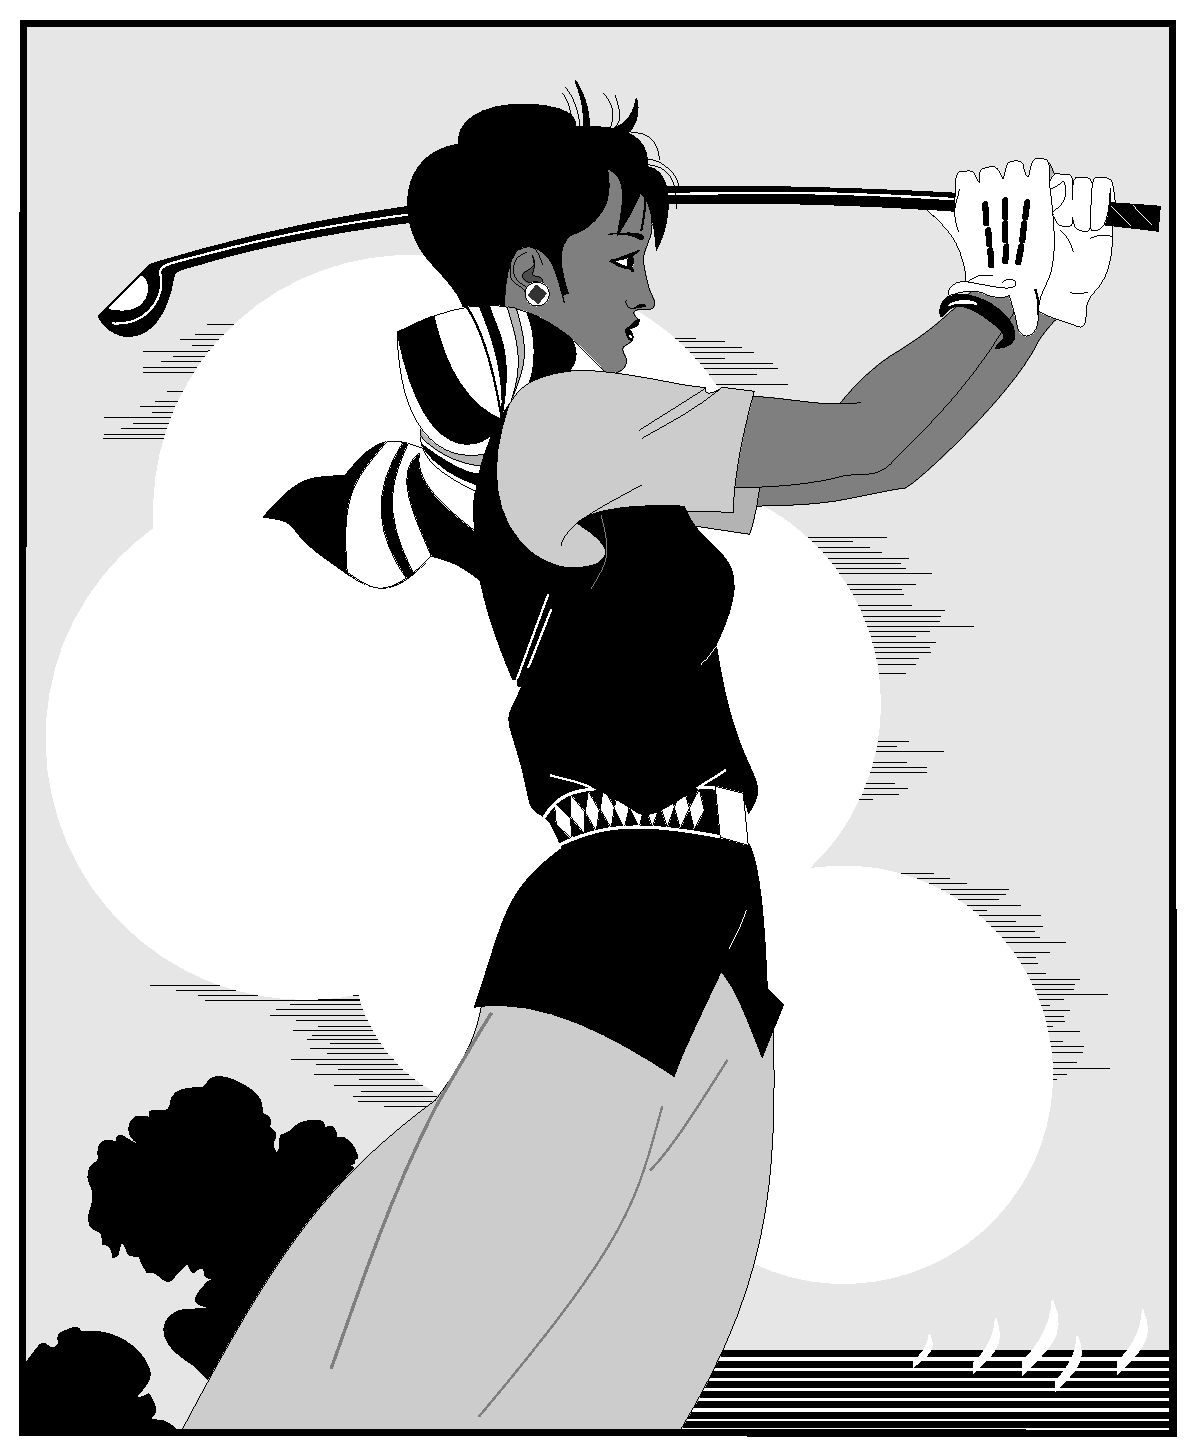
\includegraphics[width = 0.4\textwidth]{golfer}
%\bicaption[golfer5]{}{\xiaosi[0]打高尔夫球的人}{Fig.$\!$}{The person playing golf}\vspace{-1em}
\caption{\xiaosi[0]打高尔夫球的人}
\label{fig:appA}
\end{figure}

附录中\equref{eq:appA}:
\begin{align}
a & = b \times c \\
E & = m c^2
\label{eq:appA}
\end{align}

%   % !TEX root = ../main.tex

% 附录B
\chapter{这个星球上最好的免费Linux软件列表}[List of the Best Linux Software in our Planet]
\section{系统}

\href{http://fvwm.org/}{FVWM 自从上世纪诞生以来,此星球最强大的窗口管理器。}
推荐基于FVWM的桌面设计hifvwm:\href{https://github.com/dustincys/hifvwm}{https://github.com/dustincys/hifvwm}。

\subsection{hifvwm的优点}

\begin{enumerate}
	\item 即使打开上百个窗口也不会“蒙圈”。计算机性能越来越强大,窗口任务的管理必须要升级到打怪兽级别。
	\item 自动同步Bing搜索主页的壁纸。每次电脑开机,午夜零点自动更新,用户
		也可以手动更新,从此审美再也不疲劳。
	\item 切换窗口自动聚焦到最上面的窗口。使用键盘快捷键切换窗口时候,减少
		操作过程,自动聚焦到目标窗口。这一特性是虚拟窗口必须的人性化设
		计。
	\item 类似window右下角的功能的最小化窗口来显示桌面的功能此处类似
		win7/win10,实现在一个桌面之内操作多个任务。
	\item 任务栏结合标题栏。采用任务栏和标题栏结合,节省空间。
	\item 同类窗口切换。可以在同类窗口之内类似alt-tab的方式切换。
	\item ……
\end{enumerate}

\section{其他}

\href{https://orgmode.org/}{orgmode,最强大的笔记系统,从来没有之一。}

\href{https://www.jianguoyun.com/}{坚果云,国内一款支持WebDav的云盘系统,国内真正的云盘没有之一。}

\section{vim}
实现中英文每一句一行,以及实现每一句折叠断行的简单正则式,tex源码更加乖乖。
\begin{lstlisting}
vnoremap <leader>fae J:s/[.!?]\zs\s\+/\="\r".matchstr(getline('.'), '^\s*')/g<CR>
vnoremap <leader>fac J:s/[。!?]/\=submatch(0)."\n".matchstr(getline('.'), '^\s*')/g<CR>
vnoremap <leader>fle :!fmt -80 -s<CR>
\end{lstlisting}

% \end{appendix}

% % 发表文章
% % !Mode:: "TeX:UTF-8" 
\begin{publication}
\noindent\textbf{发表的相关论文}
\begin{publist}
\item	XXX,XXX. Static Oxidation Model of Al-Mg/C Dissipation Thermal Protection Materials[J]. Rare Metal Materials and Engineering, 2010, 39(Suppl. 1): 520-524.(SCI~收录,IDS号为~669JS,IF=0.16)
\item XXX,XXX. 精密超声振动切削单晶铜的计算机仿真研究[J]. 系统仿真学报,2007,19(4):738-741,753.(EI~收录号:20071310514841)
\item XXX,XXX. 局部多孔质气体静压轴向轴承静态特性的数值求解[J]. 摩擦学学报,2007(1):68-72.(EI~收录号:20071510544816)
\item XXX,XXX. 硬脆光学晶体材料超精密切削理论研究综述[J]. 机械工程学报,2003,39(8):15-22.(EI~收录号:2004088028875)
\item XXX,XXX. 基于遗传算法的超精密切削加工表面粗糙度预测模型的参数辨识以及切削参数优化[J]. 机械工程学报,2005,41(11):158-162.(EI~收录号:2006039650087)
\item XXX,XXX. Discrete Sliding Mode Cintrok with Fuzzy Adaptive Reaching Law on 6-PEES Parallel Robot[C]. Intelligent System Design and Applications, Jinan, 2006: 649-652.(EI~收录号:20073210746529)
\end{publist}

\noindent\textbf{(二)申请及已获得的专利(无专利时此项不必列出)}
\begin{publist}
\item XXX,XXX. 一种温热外敷药制备方案:中国,88105607.3[P]. 1989-07-26.
\end{publist}

\noindent\textbf{(三)参与的科研项目及获奖情况}
\begin{publist}
\item	XXX,XXX. XX~气体静压轴承技术研究, XX~省自然科学基金项目.课题编号:XXXX.
\item XXX,XXX. XX~静载下预应力混凝土房屋结构设计统一理论. 黑江省科学技术二等奖, 2007.
\end{publist}
%\vfill
%\hangafter=1\hangindent=2em\noindent
%\setlength{\parindent}{2em}
\end{publication}


% % 索引
% % \begin{ceindex}
  %如果想要手动加索引,注释掉以下这一样,用wordlist环境
\printsubindex*
\end{ceindex}


% % 授权
% \authorization

% % 授权页为扫描的PDF文件(scan.pdf),与上面的命令互斥
% % \authorization[scan.pdf]

% % 致谢
% % !TEX root = ../main.tex

% 致谢
\begin{acknowledgements}
衷心感谢导师~XXX~教授对本人的精心指导。他的言传身教将使我终生受益。

……

感谢哈深\LaTeX{}论文模板\hitszthesis\ !

\end{acknowledgements}


% % 个人简介
% % !TEX root = ../main.tex

% 个人简历
\begin{resume}

  XXXX~年~XX~月~XX~日出生于~XXXX。

  XXXX~年~XX~月考入~XX~大学~XX~院(系)XX~专业,XXXX~年~XX~月本科毕业并获得~XX~学学士学位。

  XXXX~年~XX~月------XXXX~年~XX~月在~XX~大学~XX~院(系)XX~学科学习并获得~XX~学硕士学位。

  XXXX~年~XX~月------XXXX~年~XX~月在~XX~大学~XX~院(系)XX~学科学习并获得~XX~学博士学位。

  获奖情况:如获三好学生、优秀团干部、X~奖学金等(不含科研学术获奖)。

  工作经历:

  \songti\textbf{(除全日制硕士生以外,其余学生均应增列此项。个人简历一般应包含教育经历和工作经历。)}

\end{resume}


%%%% \end{硕博书序}


% 结束文档撰写
\end{document}
%%=============================================

% Local Variables:
% TeX-engine: xetex
% End:
